%Began 29 August 2017 --- Memorial of the Passion and Death of St. John the Baptist 
\documentclass[letterpaper,x11names,svgnames,10pt]{article}
\usepackage{amsmath}
\usepackage{hyperref}
% the \hypersetup{keyvals} commented out below is stored in an external hyperref.cfg file
% to enable the pagebackref=true option
%\hypersetup{%dvips, % not needed for  pdflatex
%	pagebackref=true,
%	pdfauthor={Iam The Author},
%	hyperfigures,
%	bookmarks=true,
%	bookmarksnumbered=true,
%	bookmarksopen=true,
%	colorlinks=true, %if true, link borders absent
%	pdfborder={1 1 1},
%	citecolor=blue,
%	linkcolor=blue,
%	urlcolor=blue,
%}
\usepackage{url}
\usepackage{svg}
\usepackage{graphicx}
\usepackage{xcolor}
\usepackage{float}
\usepackage{natbib}

\topmargin -0.50in
\oddsidemargin 0.25in
\textwidth 6.50in
\textheight 9.00in

%%%-------------------------------------------
%%% TO BE EDITED FOR EACH NEW VOLUME GENERATED 
%%%-------------------------------------------
	\def\authorName{I Am The Author}
	\def\authorFirstMidNameInit{I.\ T.\ }
	\def\authorLastName{Author}
	\def\dateGenerated{29 August 2017}
	\def\volNumber{I}
%%%-------------------------------------------
%%%

\def\uline{\underline}
%\definecolor{orange}{rgb}{1,0.5,0} % RGB
%\definecolor{light-gray}{gray}{0.95} % shades
%\definecolor{orange}{cmyk}{0,0.5,1,0} % CMYK

\newcommand{\HRule}{\rule{\linewidth}{0.5mm}}

\setlength{\parindent}{0pt}

\DeclareGraphicsExtensions{.pdf,.png}

\setcitestyle{authoryear,round,comma,aysep={,},yysep={,},notesep={, }}

\title{\textsc{Musical Dice Games Minuets \volNumber}}
\author{\textsc{\authorFirstMidNameInit \authorLastName}}
\date{\textsc{\dateGenerated}}
% -----

\begin{document}

% Book Cover
% File name: mdgBooSVGV1-cover.tex
% Purpose: Book Cover
% InstructionL Should be \input{.} just after \begin{document}
{
\topmargin 0.00in
\oddsidemargin 0.45in
\textwidth 8.50in
\textheight 11.50in
\thispagestyle{empty}

\begin{titlepage}

\begin{picture}(0,0)%
\linethickness{67.00pt}
\color{blue!22!black}
\put(-105,85){\line(1,0){6477}}
\put(-105,-612){\includegraphics[clip=true,trim=0.00in 0.65in 0.25in 1.525in, height=11.75in,width=8.60in,keepaspectratio]%
	{../images/FrontCover}}
\put(-105,-645){\line(1,0){6477}}
\end{picture}

\vspace{-1.50in}

\begin{center}
	\LARGE\textbf{\color{white} Wonders of the Musical World Series}
\end{center}

\vspace*{2.5\baselineskip}
\begin{center} \Huge\textbf{\color{LightGoldenrod!1!Gold}\em Musical Dice Games Minuets \volNumber}
\end{center}

\begin{center}
	\Large\textbf{\color{LightGoldenrod!1!Gold}\em based on  Musikalisches W\"{u}rfelspiel K.\ 516f (1787)}
\end{center}

\begin{center}
	\LARGE\textbf{\color{LightGoldenrod!50!Gold}\em compiled by \authorFirstMidNameInit \authorLastName}
\end{center}

\vfill
\begin{center}
	\LARGE\textbf{\color{white}\em Libre Edition Press \\ \vspace{-0.25in}}
\end{center}
\end{titlepage}
}




\newpage
% Title Page
{
	${}_{}$\\
	\vspace{1.00in}	
	\thispagestyle{empty}
	\begin{center}
		\HRule \\[0.4cm]
		{ \huge \bfseries Musical Dice Games Minuets \volNumber} \\[0.2cm]
		{\large based on {\em Musikalisches W\"{u}rfelspiel, K.\ 516f (1787)} }\\[0.2cm]
		\HRule \\[1.5cm]
		% Author and supervisor
		\begin{minipage}{0.4\textwidth}
			\begin{flushleft} \large
				\emph{Author:}\\
				\authorFirstMidNameInit \textsc{\authorLastName}
			\end{flushleft}
		\end{minipage}
		\begin{minipage}{0.4\textwidth}
			\begin{flushright} \large
				\emph{Supervisor:} \\
				Dr. Communio \textsc{Sanctorum}
			\end{flushright}
		\end{minipage}
		\vfill
		% Bottom of the page
		{\textsc{\Large Wonders of the Musical World Series}}  \\[0.2cm] 
		\includegraphics*[width=0.15\linewidth]{../images/1.png}\\ 
		{\large Libre Edition Press \\
		         \dateGenerated }\\
		\vspace{2.50in}
	\end{center}
	\newpage
	
	%\maketitle
	
	\tableofcontents\label{tabofcon}
	
	%\extrafloats{182}

\section[Introduction]{Introduction\footnote{The information contained in the introduction were culled from the following online resources:
	\citet{wiki_mw2017},
	\url{https://opus-infinity.org/}, and 
	\hyperref{https://www.sciencenews.org/article/mozarts-melody-machine-0}{}{}{Mozart's Melody Machine} \citep*{peterson2001}
	}
}
	\begin{center}
	\begin{minipage}{0.4\textwidth}
	\begin{flushleft}
		\begin{center}
			``ANLEITUNG\\
			Walzer oder Schleifer mit zwei\\
			W\"{u}rfeln zu componiren, so\\
			viele man will, ohne\\
			etwas von der Musik\\
			oder Composition\\
			zu verstehen."\\
		\end{center}
	\end{flushleft}
	\end{minipage}
	\begin{minipage}{0.4\textwidth}
	\begin{flushright}
		\begin{center}
		``INSTRUCTION\\
		To compose without the least knowledge\\
		of Music so much German Walzer or Schleifer as\\
		one pleases, by throwing a\\
		certain Number with two Dice."
	\end{center}
	\end{flushright}
	\end{minipage}
	\end{center}

Thus run the German title and its English translation of the most well-known of Musical Dice Games (MDG).  Rightly and interestingly so, as the Instructions provided in the published work allow a non-professional musician to generate (``compose") as nearly as 398 trillions of MDG minuets (more precisely, $11^{14} = 397,749,833,583,241$).\\  

A {\it Musikalisches W\"{u}rfelspiel} (German for ``musical dice game" or MDG) is a system for randomly ``generating" (e.g., by using a die or two dice) musical compositions from precomposed options and was quite popular throughout Western Europe in the 18th century.  The earliest known MDG is Johann Philipp Kirnberger's {\em Der allezeit fertige Menuetten und Polonaisencomponist (1st ed.\ 1757; rev.\ 2nd ed.\ 1783)} (translated from German as ``The Ever-Ready Minuet and Polonaise Composer").  Other well-known composers that are to known to have composed a MDG are C.P.E.\ Bach ({\em Einfall, einen doppelten Contrapunct in der Octave von sechs Tacten zu machen, ohne die Regeln davon zu wissen (1758)}; translated from German as ``A method for making six bars of double counterpoint at the octave without knowing the rules") and Abb\'{e} Maximillian Stadler ({\em Table pour composer des minuets et des Trios \`{a} la infinie; avec deux dez \`{a} jouer (1780)}; translated from French as ``A table for composing minuets and trios to infinity, by playing with two dice"). \\

{\it Musikalisches W\"{u}rfelspiel K. 516f (1787)}, another title for the most famous of MDGs, was first published by J.J. Hummel in 1793 in Berlin, and was republished in 1796 by Nikolaus Simrock in Bonn (as K. 294d or K. Anh. C 30.01).  Simrock attributed this work, which is also known under the title of {\em Anleitung zum Componieren von Walzern so viele man will vermittelst zweier Würfel, ohne etwas von der Musik oder Composition zu verstehen} (German for ``Instructions for the composition of as many waltzes as one desires with two dice, without understanding anything about music or composition"), to Wolfgang Amadeus Mozart and it may have been based on Mozart's manuscript K. 516f, written in 1787, consisting of numerous two-bar fragments of music, that appear to be some kind of game or system for constructing music out of two-bar fragments, but contains no instructions nor hints as to the use of dice.  An online article by Hideo Noguchi offers a possible explanation for this attribution. \\

This book is a collection of 250 Musical Dice Games (MDG) minuets generated according to the rules given in {\it Musikalisches W\"{u}rfelspiel K. 516f}.  The scores of the generated minuets, that were initially written in using the \texttt{abc} environment of Chris Walshaw, were converted to Scalar Vector Image (SVG) images and were then pre-processed with Inkscape to be included in \LaTeX\ to produce this book.


\section{\em Musikalisches W\"{u}rfelspiel K.\ 516f}

\subsection{Rules}

The Rules provided in {\em Musikalisches W\"{u}rfelspiel} generate MDG minuets consisting of 16 measures.  The first eight (8) measures are played then repeated, with a variation on the 8th measure on the repeat leading to the 9th measure.  The last eight measures are then similarly played with the 16th measure remaining the same even on the repeat. \\

The following Rules are followed for generating each minuet:
\begin{enumerate}
	\item [1.] For each measure from the first to the 16th, two dice are tossed and the sum of the two faces that come up are obtained.  Hence, 16 two-dice tosses (with possible outcomes from the set \{2, 3, 4, 5, 6, 7, 8, 9, 10, 11, 12\}, one two-dice toss for each measure, are needed to generate a minuet.   
	\item [2.] Table~\ref{fig:0tab1} is then used to determine which measure number from the Table of Measures (Figures~\ref{fig:meas1} to \ref{fig:meas4}) is to be used for obtaining the notes for the particular measure of the minuet corresponding to the outcome of the two-dice toss.  The possible outcomes of a two-dice toss (2 to 12) are given on the left-hand side of Table~\ref{fig:0tab1}, while the measure numbers of the minuet-to-be-generated are given on the top of that table.
	\item [3.]  For example, suppose for measure 1, the outcome of the two-dice toss is 5.  If we now look for measure number 1 at the top of Table~\ref{fig:0tab1} and for the outcome 5 on the left-hand side of that table, we obtain 40 as the measure number of the Table of Measures (Figures~\ref{fig:meas1} to \ref{fig:meas4}) to be used for obtaining the notes to be played for the first measure of the minuet to be generated.  An outcome of 11 for the two-dice toss for measure nine (9) of the minuet to be constructed leads us to obtain the notes from measure 102 of the Table of Measures.
\end{enumerate}   


\subsection{Table for finding Measure Number from Table of Measures}
The table given here (Table~\ref{fig:0tab1}) combines the two tables given on page 2 of {\it Musikalisches W\"{u}rfelspiel K. 516f (1787)} but the contents are exactly as given there.  The leftmost column contains the possible two-dice outcomes while the topmost row contains the measure number for the MDG minuet to be generated.

\begin{table}[H]
	\centering
	\begin{tabular}{c}
		\centering
		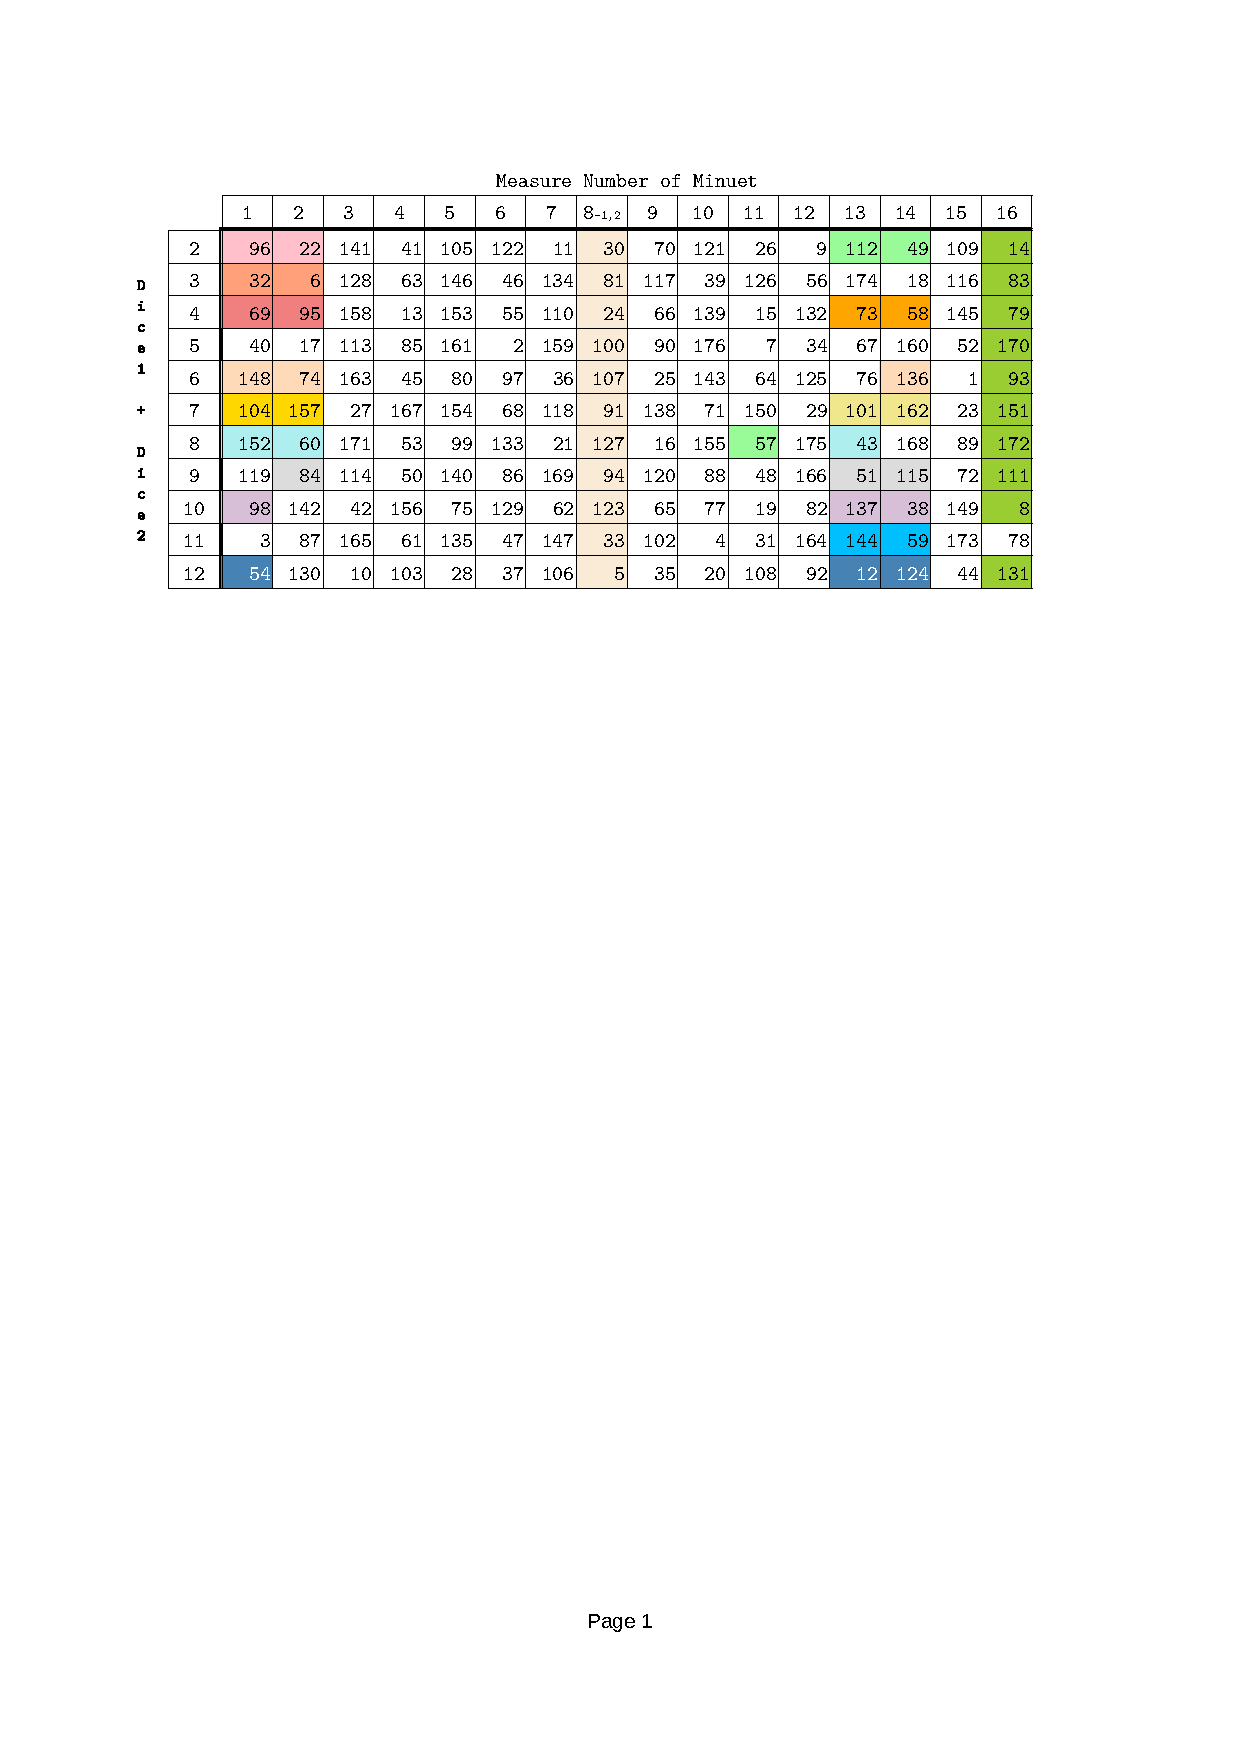
\includegraphics[clip=true,trim=0.90in 7.75in 1.25in 1.00in,scale=0.90]{12TAB}
	\end{tabular}
	\caption{Measure number to be looked-up in the Table of Measures (see Figures~\ref{fig:meas1}, \ref{fig:meas2}, \ref{fig:meas3}, and \ref{fig:meas4}) corresponding to each two-dice outcome per measure of the minuet.}
	\label{fig:0tab1}
\end{table}

\nopagebreak[4]
\subsection{Table of Measures}

\addcontentsline{toc}{subsection}{\hspace*{0.25in} K516f page 1 of measures}
\begin{figure}[H]
	\centering
	\def\svgwidth{0.975\columnwidth}
	\input{abcmdg-k516f001.pdf_tex}
	\caption{Table of Measures (Part I)}
	\label{fig:meas1}
\end{figure}

\newpage
${}_{}$\\
\vspace{0.10in}
\addcontentsline{toc}{subsection}{\hspace*{0.25in} K516f page 2 of measures}
\begin{figure}[H]
	\centering
	\def\svgwidth{0.975\columnwidth}
	\input{abcmdg-k516f002.pdf_tex}
	\caption{Table of Measures (Part II)}
	\label{fig:meas2}
\end{figure}

\newpage
${}_{}$\\
\vspace{0.10in}
\addcontentsline{toc}{subsection}{\hspace*{0.25in} K516f page 3 of measures}	
\begin{figure}[H]
	\centering
	\def\svgwidth{0.975\columnwidth}
	\input{abcmdg-k516f003.pdf_tex}
	\caption{Table of Measures (Part III)}
	\label{fig:meas3}
\end{figure}

\newpage
${}_{}$\\
\vspace{0.10in}
\addcontentsline{toc}{subsection}{\hspace*{0.25in} K516f page 4 of measures}
\begin{figure}[H]
	\centering
	\def\svgwidth{0.975\columnwidth}
	\input{abcmdg-k516f004.pdf_tex}
	\caption{Table of Measures (Part IV)}
	\label{fig:meas4}
\end{figure}


\newpage
\section{Related Links}
The following are very interesting sites in that they allow the online rendering of MDGs:
\begin{itemize}
	\item  \hyperref{https://marian-aldenhoevel.de/mozart/}{}{}{Mozart} - A site maintained by Marian Aldenh\"{o}vel allows the visitor to generate a MDG (user-specified or randomly-generated) and the corresponding audio ({\tt midi, wav}) and image files ({\tt pdf, png}) based on {\em Musikalisches W\"{u}rferspiel, K.\ 516f}.
	
	\item \hyperref{https://opus-infinity.org}{}{}{Opus Infinity} - Collaborative work of Robbert Harms, Hein Moors, and Suus van Petegem whose goal is to unravel the mystery behind the tables used for generating MDGs.  Site visitors can generate MDGs based on works of Kirnberger, Mozart, Stadler/Haydn, and Bach.  Corresponding audio files ({\tt mid, ogg,} and/or {\tt mp3}) and image files ({\tt pdf} or {\tt png}) are also made available for listening, viewing, or downloading.
	
	\item  \hyperref{http://sunsite.univie.ac.at/Mozart/dice/}{}{}{Mozart} - A site maintained by John Chuang that allows the site visitor to generate MDGs based on the work of Stadler/Haydn.
 	
 	\item \hyperref{http://www.amaranthpublishing.com/MozartDiceGame.htm}{}{}{\tt mozart.zip} -  This is a Windows software (\textcopyright 1995 VisionSoft) by John Chuang and Stephen Goodwin that generates MDG based on input from user and is available for {\it free} from  \hyperref{http://www.amaranthpublishing.com/MozartDiceGame.htm}{}{}{Amaranth Publishing}.  
 	
 	\item \hyperref{(http://www.asahi-net.or.jp/\~rb5h-ngc/e/k516f.htm}{}{}{``Mozart - Musical Game in C K. 516f,"}	Mozart Studies Online - The site of Hideo Noguchi that offers an explanation linking {\em Musikalisches W\"{u}rferspiel, K.\ 516f}, and  {\em K.\ 294d (K.\ Anh.\ C 30.01)}. 
\end{itemize}

\section{Acknowledgments}
My sincerest gratitude to Chris Walshaw et al. for the \hyperref{http://www.abcnotation.com/}{}{}{ABC music notation}; Jean-Francois Moine for \hyperref{http://moinejf.free.fr/}{}{}{\tt abcm2ps} and the accompanying examples, templates, and pointers for the appropriate use of these resources; Guido Gonzato for the \hyperref{http://abcplus.sourceforge.net/}{}{}{ABC Plus Project} and the \hyperref{http://abcplus.sourceforge.net/#abcMIDI}{}{}{{\tt abcmidi} resources} available there, more especially for the ABC resource book {\em Making Music with ABC 2}; James R. Allwright and Seymour Shlien for \hyperref{http://abc.sourceforge.net/abcMIDI}{}{}{\tt abcmidi} source and binaries; \hyperref{https://artifex.com/}{}{}{Artifex, Inc.} for Ghostscript v.9.06 (includes the {\tt ps2pdf} converter); \hyperref{https://www.inkscape.org/}{}{}{Inkscape v.0.48.5} for the tool for converting SVGs to PDFs for inclusion into \LaTeX\ documents; and \hyperref{https://tex.stackexchange.com/users/632/martin-h}{}{}{\tt User:Martin H} for his \hyperref{https://tex.stackexchange.com/questions/2099/how-to-include-svg-diagrams-in-latex}{}{}{reply} to a TeX/LaTeX Stack Exchange question on including SVGs into \LaTeX\ documents. Special thanks also to the \hyperref{http://imslp.org/}{}{}{International Music Score Library Project (IMSLP)} for making available the score for {\em Musikalisches W\"{u}rfelspiel, K.516f} and \hyperref{http://www.amaranthpublishing.com/MozartDiceGame.htm}{}{}{Amaranth Publishing} for a copy of {\tt mozart.zip}. Ditto to Machtelt Garrels for the book \hyperref{http://tldp.org/LDP/Bash-Beginners-Guide/html/Bash-Beginners-Guide.html}{}{}{Bash Guide for Beginners}, Vivek Gite for the book \hyperref{http://www.freeos.com/guides/lsst/}{}{}{Linux Script Shell Tutorial}, and Steve Parker for the \hyperref{http://steve-parker.org/sh/cheatsheet.pdf}{}{}{Unix/Linux Shell Cheatsheet}. John Fogarty's GitHub Site: \hyperref{https://github.com/jfogarty/latex-createspace-bookcover}{}{}{Latex CreateSpace BookCover} and Peter Wilson's reply in TeX/LaTeX Stack Exchange on \hyperref{https://tex.stackexchange.com/questions/17579/how-can-i-design-a-book-cover}{}{}{designing a book cover}, were sources of ideas, information, and materials for creating the book cover and title page, thanks to both of them; \hyperref{http://www.libreoffice.org/}{}{}{LibreOffice Calc} for its use in the image creation of the book cover.  Many thanks, too, to the \hyperref{https://www.debian.org}{}{}{Debian Project} for the Debian 8 (Jessie) GNU/Linux OS, \hyperref{http://www.tug.org/texlive/}{}{}{TeXLive} for providing the \TeX\ distribution,  and \hyperref{https://github.com}{}{}{GitHub} for its generosity in providing space for \hyperref{https://github.com/justineuro/mdgBookSVG\_1}{}{}{the project}.  

\newpage
\section{Selected Minuets}
{
\topmargin -0.75in
\textheight 9,15 in
	\addcontentsline{toc}{subsection}{10-10-6-3-5-5-11-7-8-12-5-3-7-6-6-4}
\begin{figure}[H]
	\centering
	\def\svgwidth{\columnwidth}
	\input{K516f-10-10-6-3-5-5-11-7-8-12-5-3-7-6-6-4001.pdf_tex}
\end{figure}
\nopagebreak[4]
{\footnotesize For audio (midi): \hyperref{./K516f-10-10-6-3-5-5-11-7-8-12-5-3-7-6-6-4.mid}{}{}{K516f-10-10-6-3-5-5-11-7-8-12-5-3-7-6-6-4.mid}}

\addcontentsline{toc}{subsection}{10-10-7-8-6-11-3-6-5-11-4-5-4-11-10-10}
\begin{figure}[H]
	\centering
	\def\svgwidth{\columnwidth}
	\input{K516f-10-10-7-8-6-11-3-6-5-11-4-5-4-11-10-10001.pdf_tex}
\end{figure}
\nopagebreak[4]
{\footnotesize For audio (midi): \hyperref{./K516f-10-10-7-8-6-11-3-6-5-11-4-5-4-11-10-10.mid}{}{}{K516f-10-10-7-8-6-11-3-6-5-11-4-5-4-11-10-10.mid}}

\addcontentsline{toc}{subsection}{10-10-8-2-9-6-8-11-11-12-7-12-4-7-9-7}
\begin{figure}[H]
	\centering
	\def\svgwidth{\columnwidth}
	\input{K516f-10-10-8-2-9-6-8-11-11-12-7-12-4-7-9-7001.pdf_tex}
\end{figure}
\nopagebreak[4]
{\footnotesize For audio (midi): \hyperref{./K516f-10-10-8-2-9-6-8-11-11-12-7-12-4-7-9-7.mid}{}{}{K516f-10-10-8-2-9-6-8-11-11-12-7-12-4-7-9-7.mid}}

\addcontentsline{toc}{subsection}{10-11-3-11-9-12-8-9-5-7-9-9-3-9-8-3}
\begin{figure}[H]
	\centering
	\def\svgwidth{\columnwidth}
	\input{K516f-10-11-3-11-9-12-8-9-5-7-9-9-3-9-8-3001.pdf_tex}
\end{figure}
\nopagebreak[4]
{\footnotesize For audio (midi): \hyperref{./K516f-10-11-3-11-9-12-8-9-5-7-9-9-3-9-8-3.mid}{}{}{K516f-10-11-3-11-9-12-8-9-5-7-9-9-3-9-8-3.mid}}

\addcontentsline{toc}{subsection}{10-11-4-2-6-7-3-4-9-8-5-10-7-12-9-10}
\begin{figure}[H]
	\centering
	\def\svgwidth{\columnwidth}
	\input{K516f-10-11-4-2-6-7-3-4-9-8-5-10-7-12-9-10001.pdf_tex}
\end{figure}
\nopagebreak[4]
{\footnotesize For audio (midi): \hyperref{./K516f-10-11-4-2-6-7-3-4-9-8-5-10-7-12-9-10.mid}{}{}{K516f-10-11-4-2-6-7-3-4-9-8-5-10-7-12-9-10.mid}}

\addcontentsline{toc}{subsection}{10-11-8-7-3-8-3-3-4-6-7-6-11-12-12-3}
\begin{figure}[H]
	\centering
	\def\svgwidth{\columnwidth}
	\input{K516f-10-11-8-7-3-8-3-3-4-6-7-6-11-12-12-3001.pdf_tex}
\end{figure}
\nopagebreak[4]
{\footnotesize For audio (midi): \hyperref{./K516f-10-11-8-7-3-8-3-3-4-6-7-6-11-12-12-3.mid}{}{}{K516f-10-11-8-7-3-8-3-3-4-6-7-6-11-12-12-3.mid}}

\addcontentsline{toc}{subsection}{10-12-10-8-2-11-9-9-10-3-10-4-6-10-4-2}
\begin{figure}[H]
	\centering
	\def\svgwidth{\columnwidth}
	\input{K516f-10-12-10-8-2-11-9-9-10-3-10-4-6-10-4-2001.pdf_tex}
\end{figure}
\nopagebreak[4]
{\footnotesize For audio (midi): \hyperref{./K516f-10-12-10-8-2-11-9-9-10-3-10-4-6-10-4-2.mid}{}{}{K516f-10-12-10-8-2-11-9-9-10-3-10-4-6-10-4-2.mid}}

\addcontentsline{toc}{subsection}{10-12-12-12-10-5-10-7-5-3-5-3-11-12-3-2}
\begin{figure}[H]
	\centering
	\def\svgwidth{\columnwidth}
	\input{K516f-10-12-12-12-10-5-10-7-5-3-5-3-11-12-3-2001.pdf_tex}
\end{figure}
\nopagebreak[4]
{\footnotesize For audio (midi): \hyperref{./K516f-10-12-12-12-10-5-10-7-5-3-5-3-11-12-3-2.mid}{}{}{K516f-10-12-12-12-10-5-10-7-5-3-5-3-11-12-3-2.mid}}

\addcontentsline{toc}{subsection}{10-12-3-10-8-4-2-12-10-5-11-10-7-7-9-10}
\begin{figure}[H]
	\centering
	\def\svgwidth{\columnwidth}
	\input{K516f-10-12-3-10-8-4-2-12-10-5-11-10-7-7-9-10001.pdf_tex}
\end{figure}
\nopagebreak[4]
{\footnotesize For audio (midi): \hyperref{./K516f-10-12-3-10-8-4-2-12-10-5-11-10-7-7-9-10.mid}{}{}{K516f-10-12-3-10-8-4-2-12-10-5-11-10-7-7-9-10.mid}}

\addcontentsline{toc}{subsection}{10-12-3-9-8-10-3-9-4-3-7-3-4-8-3-10}
\begin{figure}[H]
	\centering
	\def\svgwidth{\columnwidth}
	\input{K516f-10-12-3-9-8-10-3-9-4-3-7-3-4-8-3-10001.pdf_tex}
\end{figure}
\nopagebreak[4]
{\footnotesize For audio (midi): \hyperref{./K516f-10-12-3-9-8-10-3-9-4-3-7-3-4-8-3-10.mid}{}{}{K516f-10-12-3-9-8-10-3-9-4-3-7-3-4-8-3-10.mid}}

\addcontentsline{toc}{subsection}{10-12-5-6-10-6-5-6-7-5-7-2-4-3-3-9}
\begin{figure}[H]
	\centering
	\def\svgwidth{\columnwidth}
	\input{K516f-10-12-5-6-10-6-5-6-7-5-7-2-4-3-3-9001.pdf_tex}
\end{figure}
\nopagebreak[4]
{\footnotesize For audio (midi): \hyperref{./K516f-10-12-5-6-10-6-5-6-7-5-7-2-4-3-3-9.mid}{}{}{K516f-10-12-5-6-10-6-5-6-7-5-7-2-4-3-3-9.mid}}

\addcontentsline{toc}{subsection}{10-12-7-8-3-5-7-6-2-9-2-11-12-2-6-3}
\begin{figure}[H]
	\centering
	\def\svgwidth{\columnwidth}
	\input{K516f-10-12-7-8-3-5-7-6-2-9-2-11-12-2-6-3001.pdf_tex}
\end{figure}
\nopagebreak[4]
{\footnotesize For audio (midi): \hyperref{./K516f-10-12-7-8-3-5-7-6-2-9-2-11-12-2-6-3.mid}{}{}{K516f-10-12-7-8-3-5-7-6-2-9-2-11-12-2-6-3.mid}}

\addcontentsline{toc}{subsection}{10-2-8-3-9-6-11-8-2-12-12-9-6-3-6-9}
\begin{figure}[H]
	\centering
	\def\svgwidth{\columnwidth}
	\input{K516f-10-2-8-3-9-6-11-8-2-12-12-9-6-3-6-9001.pdf_tex}
\end{figure}
\nopagebreak[4]
{\footnotesize For audio (midi): \hyperref{./K516f-10-2-8-3-9-6-11-8-2-12-12-9-6-3-6-9.mid}{}{}{K516f-10-2-8-3-9-6-11-8-2-12-12-9-6-3-6-9.mid}}

\addcontentsline{toc}{subsection}{10-2-9-5-6-6-10-11-11-10-8-12-12-6-5-10}
\begin{figure}[H]
	\centering
	\def\svgwidth{\columnwidth}
	\input{K516f-10-2-9-5-6-6-10-11-11-10-8-12-12-6-5-10001.pdf_tex}
\end{figure}
\nopagebreak[4]
{\footnotesize For audio (midi): \hyperref{./K516f-10-2-9-5-6-6-10-11-11-10-8-12-12-6-5-10.mid}{}{}{K516f-10-2-9-5-6-6-10-11-11-10-8-12-12-6-5-10.mid}}

\addcontentsline{toc}{subsection}{10-3-11-3-3-5-3-6-8-6-7-12-10-10-11-5}
\begin{figure}[H]
	\centering
	\def\svgwidth{\columnwidth}
	\input{K516f-10-3-11-3-3-5-3-6-8-6-7-12-10-10-11-5001.pdf_tex}
\end{figure}
\nopagebreak[4]
{\footnotesize For audio (midi): \hyperref{./K516f-10-3-11-3-3-5-3-6-8-6-7-12-10-10-11-5.mid}{}{}{K516f-10-3-11-3-3-5-3-6-8-6-7-12-10-10-11-5.mid}}

\addcontentsline{toc}{subsection}{10-3-2-9-9-12-9-2-3-7-12-10-4-6-7-5}
\begin{figure}[H]
	\centering
	\def\svgwidth{\columnwidth}
	\input{K516f-10-3-2-9-9-12-9-2-3-7-12-10-4-6-7-5001.pdf_tex}
\end{figure}
\nopagebreak[4]
{\footnotesize For audio (midi): \hyperref{./K516f-10-3-2-9-9-12-9-2-3-7-12-10-4-6-7-5.mid}{}{}{K516f-10-3-2-9-9-12-9-2-3-7-12-10-4-6-7-5.mid}}

\addcontentsline{toc}{subsection}{10-3-3-4-4-4-3-7-3-10-9-4-7-5-10-3}
\begin{figure}[H]
	\centering
	\def\svgwidth{\columnwidth}
	\input{K516f-10-3-3-4-4-4-3-7-3-10-9-4-7-5-10-3001.pdf_tex}
\end{figure}
\nopagebreak[4]
{\footnotesize For audio (midi): \hyperref{./K516f-10-3-3-4-4-4-3-7-3-10-9-4-7-5-10-3.mid}{}{}{K516f-10-3-3-4-4-4-3-7-3-10-9-4-7-5-10-3.mid}}

\addcontentsline{toc}{subsection}{10-3-4-10-7-9-10-10-6-8-5-8-5-12-3-8}
\begin{figure}[H]
	\centering
	\def\svgwidth{\columnwidth}
	\input{K516f-10-3-4-10-7-9-10-10-6-8-5-8-5-12-3-8001.pdf_tex}
\end{figure}
\nopagebreak[4]
{\footnotesize For audio (midi): \hyperref{./K516f-10-3-4-10-7-9-10-10-6-8-5-8-5-12-3-8.mid}{}{}{K516f-10-3-4-10-7-9-10-10-6-8-5-8-5-12-3-8.mid}}

\addcontentsline{toc}{subsection}{10-3-9-3-9-10-5-2-2-8-9-10-4-4-8-2}
\begin{figure}[H]
	\centering
	\def\svgwidth{\columnwidth}
	\input{K516f-10-3-9-3-9-10-5-2-2-8-9-10-4-4-8-2001.pdf_tex}
\end{figure}
\nopagebreak[4]
{\footnotesize For audio (midi): \hyperref{./K516f-10-3-9-3-9-10-5-2-2-8-9-10-4-4-8-2.mid}{}{}{K516f-10-3-9-3-9-10-5-2-2-8-9-10-4-4-8-2.mid}}

\addcontentsline{toc}{subsection}{10-3-9-7-4-6-8-5-12-4-8-4-10-8-10-6}
\begin{figure}[H]
	\centering
	\def\svgwidth{\columnwidth}
	\input{K516f-10-3-9-7-4-6-8-5-12-4-8-4-10-8-10-6001.pdf_tex}
\end{figure}
\nopagebreak[4]
{\footnotesize For audio (midi): \hyperref{./K516f-10-3-9-7-4-6-8-5-12-4-8-4-10-8-10-6.mid}{}{}{K516f-10-3-9-7-4-6-8-5-12-4-8-4-10-8-10-6.mid}}

\addcontentsline{toc}{subsection}{10-4-12-5-2-8-6-5-5-5-11-9-2-2-12-5}
\begin{figure}[H]
	\centering
	\def\svgwidth{\columnwidth}
	\input{K516f-10-4-12-5-2-8-6-5-5-5-11-9-2-2-12-5001.pdf_tex}
\end{figure}
\nopagebreak[4]
{\footnotesize For audio (midi): \hyperref{./K516f-10-4-12-5-2-8-6-5-5-5-11-9-2-2-12-5.mid}{}{}{K516f-10-4-12-5-2-8-6-5-5-5-11-9-2-2-12-5.mid}}

\addcontentsline{toc}{subsection}{10-4-12-9-8-12-2-9-9-11-5-9-7-8-8-4}
\begin{figure}[H]
	\centering
	\def\svgwidth{\columnwidth}
	\input{K516f-10-4-12-9-8-12-2-9-9-11-5-9-7-8-8-4001.pdf_tex}
\end{figure}
\nopagebreak[4]
{\footnotesize For audio (midi): \hyperref{./K516f-10-4-12-9-8-12-2-9-9-11-5-9-7-8-8-4.mid}{}{}{K516f-10-4-12-9-8-12-2-9-9-11-5-9-7-8-8-4.mid}}

\addcontentsline{toc}{subsection}{10-4-3-11-10-10-10-10-9-8-11-7-5-6-4-4}
\begin{figure}[H]
	\centering
	\def\svgwidth{\columnwidth}
	\input{K516f-10-4-3-11-10-10-10-10-9-8-11-7-5-6-4-4001.pdf_tex}
\end{figure}
\nopagebreak[4]
{\footnotesize For audio (midi): \hyperref{./K516f-10-4-3-11-10-10-10-10-9-8-11-7-5-6-4-4.mid}{}{}{K516f-10-4-3-11-10-10-10-10-9-8-11-7-5-6-4-4.mid}}

\addcontentsline{toc}{subsection}{10-4-5-12-3-4-12-11-8-4-8-2-12-2-12-12}
\begin{figure}[H]
	\centering
	\def\svgwidth{\columnwidth}
	\input{K516f-10-4-5-12-3-4-12-11-8-4-8-2-12-2-12-12001.pdf_tex}
\end{figure}
\nopagebreak[4]
{\footnotesize For audio (midi): \hyperref{./K516f-10-4-5-12-3-4-12-11-8-4-8-2-12-2-12-12.mid}{}{}{K516f-10-4-5-12-3-4-12-11-8-4-8-2-12-2-12-12.mid}}

\addcontentsline{toc}{subsection}{10-5-10-7-12-9-5-3-8-7-8-10-9-8-5-7}
\begin{figure}[H]
	\centering
	\def\svgwidth{\columnwidth}
	\input{K516f-10-5-10-7-12-9-5-3-8-7-8-10-9-8-5-7001.pdf_tex}
\end{figure}
\nopagebreak[4]
{\footnotesize For audio (midi): \hyperref{./K516f-10-5-10-7-12-9-5-3-8-7-8-10-9-8-5-7.mid}{}{}{K516f-10-5-10-7-12-9-5-3-8-7-8-10-9-8-5-7.mid}}

\addcontentsline{toc}{subsection}{10-6-11-7-7-4-3-3-5-12-12-3-4-10-11-9}
\begin{figure}[H]
	\centering
	\def\svgwidth{\columnwidth}
	\input{K516f-10-6-11-7-7-4-3-3-5-12-12-3-4-10-11-9001.pdf_tex}
\end{figure}
\nopagebreak[4]
{\footnotesize For audio (midi): \hyperref{./K516f-10-6-11-7-7-4-3-3-5-12-12-3-4-10-11-9.mid}{}{}{K516f-10-6-11-7-7-4-3-3-5-12-12-3-4-10-11-9.mid}}

\addcontentsline{toc}{subsection}{10-6-6-8-6-6-6-2-10-2-2-8-6-6-8-9}
\begin{figure}[H]
	\centering
	\def\svgwidth{\columnwidth}
	\input{K516f-10-6-6-8-6-6-6-2-10-2-2-8-6-6-8-9001.pdf_tex}
\end{figure}
\nopagebreak[4]
{\footnotesize For audio (midi): \hyperref{./K516f-10-6-6-8-6-6-6-2-10-2-2-8-6-6-8-9.mid}{}{}{K516f-10-6-6-8-6-6-6-2-10-2-2-8-6-6-8-9.mid}}

\addcontentsline{toc}{subsection}{10-7-3-12-11-4-11-6-8-7-12-5-3-4-6-6}
\begin{figure}[H]
	\centering
	\def\svgwidth{\columnwidth}
	\input{K516f-10-7-3-12-11-4-11-6-8-7-12-5-3-4-6-6001.pdf_tex}
\end{figure}
\nopagebreak[4]
{\footnotesize For audio (midi): \hyperref{./K516f-10-7-3-12-11-4-11-6-8-7-12-5-3-4-6-6.mid}{}{}{K516f-10-7-3-12-11-4-11-6-8-7-12-5-3-4-6-6.mid}}

\addcontentsline{toc}{subsection}{10-7-3-2-11-5-3-9-11-9-9-7-9-5-7-6}
\begin{figure}[H]
	\centering
	\def\svgwidth{\columnwidth}
	\input{K516f-10-7-3-2-11-5-3-9-11-9-9-7-9-5-7-6001.pdf_tex}
\end{figure}
\nopagebreak[4]
{\footnotesize For audio (midi): \hyperref{./K516f-10-7-3-2-11-5-3-9-11-9-9-7-9-5-7-6.mid}{}{}{K516f-10-7-3-2-11-5-3-9-11-9-9-7-9-5-7-6.mid}}

\addcontentsline{toc}{subsection}{10-7-9-12-12-4-6-4-9-10-4-11-4-11-12-9}
\begin{figure}[H]
	\centering
	\def\svgwidth{\columnwidth}
	\input{K516f-10-7-9-12-12-4-6-4-9-10-4-11-4-11-12-9001.pdf_tex}
\end{figure}
\nopagebreak[4]
{\footnotesize For audio (midi): \hyperref{./K516f-10-7-9-12-12-4-6-4-9-10-4-11-4-11-12-9.mid}{}{}{K516f-10-7-9-12-12-4-6-4-9-10-4-11-4-11-12-9.mid}}

\addcontentsline{toc}{subsection}{10-9-8-11-2-10-4-10-7-12-12-8-12-2-12-7}
\begin{figure}[H]
	\centering
	\def\svgwidth{\columnwidth}
	\input{K516f-10-9-8-11-2-10-4-10-7-12-12-8-12-2-12-7001.pdf_tex}
\end{figure}
\nopagebreak[4]
{\footnotesize For audio (midi): \hyperref{./K516f-10-9-8-11-2-10-4-10-7-12-12-8-12-2-12-7.mid}{}{}{K516f-10-9-8-11-2-10-4-10-7-12-12-8-12-2-12-7.mid}}

\addcontentsline{toc}{subsection}{11-10-4-5-3-9-11-4-5-12-9-6-6-7-6-5}
\begin{figure}[H]
	\centering
	\def\svgwidth{\columnwidth}
	\input{K516f-11-10-4-5-3-9-11-4-5-12-9-6-6-7-6-5001.pdf_tex}
\end{figure}
\nopagebreak[4]
{\footnotesize For audio (midi): \hyperref{./K516f-11-10-4-5-3-9-11-4-5-12-9-6-6-7-6-5.mid}{}{}{K516f-11-10-4-5-3-9-11-4-5-12-9-6-6-7-6-5.mid}}

\addcontentsline{toc}{subsection}{11-11-2-6-5-5-2-5-11-7-3-6-2-9-2-3}
\begin{figure}[H]
	\centering
	\def\svgwidth{\columnwidth}
	\input{K516f-11-11-2-6-5-5-2-5-11-7-3-6-2-9-2-3001.pdf_tex}
\end{figure}
\nopagebreak[4]
{\footnotesize For audio (midi): \hyperref{./K516f-11-11-2-6-5-5-2-5-11-7-3-6-2-9-2-3.mid}{}{}{K516f-11-11-2-6-5-5-2-5-11-7-3-6-2-9-2-3.mid}}

\addcontentsline{toc}{subsection}{11-12-3-7-12-5-6-10-11-6-9-7-3-9-12-4}
\begin{figure}[H]
	\centering
	\def\svgwidth{\columnwidth}
	\input{K516f-11-12-3-7-12-5-6-10-11-6-9-7-3-9-12-4001.pdf_tex}
\end{figure}
\nopagebreak[4]
{\footnotesize For audio (midi): \hyperref{./K516f-11-12-3-7-12-5-6-10-11-6-9-7-3-9-12-4.mid}{}{}{K516f-11-12-3-7-12-5-6-10-11-6-9-7-3-9-12-4.mid}}

\addcontentsline{toc}{subsection}{11-12-6-2-4-3-5-2-6-3-8-2-3-11-2-11}
\begin{figure}[H]
	\centering
	\def\svgwidth{\columnwidth}
	\input{K516f-11-12-6-2-4-3-5-2-6-3-8-2-3-11-2-11001.pdf_tex}
\end{figure}
\nopagebreak[4]
{\footnotesize For audio (midi): \hyperref{./K516f-11-12-6-2-4-3-5-2-6-3-8-2-3-11-2-11.mid}{}{}{K516f-11-12-6-2-4-3-5-2-6-3-8-2-3-11-2-11.mid}}

\addcontentsline{toc}{subsection}{11-12-6-8-4-12-12-3-10-3-2-10-2-9-2-3}
\begin{figure}[H]
	\centering
	\def\svgwidth{\columnwidth}
	\input{K516f-11-12-6-8-4-12-12-3-10-3-2-10-2-9-2-3001.pdf_tex}
\end{figure}
\nopagebreak[4]
{\footnotesize For audio (midi): \hyperref{./K516f-11-12-6-8-4-12-12-3-10-3-2-10-2-9-2-3.mid}{}{}{K516f-11-12-6-8-4-12-12-3-10-3-2-10-2-9-2-3.mid}}

\addcontentsline{toc}{subsection}{11-12-6-9-3-10-8-2-11-9-10-2-3-7-3-5}
\begin{figure}[H]
	\centering
	\def\svgwidth{\columnwidth}
	\input{K516f-11-12-6-9-3-10-8-2-11-9-10-2-3-7-3-5001.pdf_tex}
\end{figure}
\nopagebreak[4]
{\footnotesize For audio (midi): \hyperref{./K516f-11-12-6-9-3-10-8-2-11-9-10-2-3-7-3-5.mid}{}{}{K516f-11-12-6-9-3-10-8-2-11-9-10-2-3-7-3-5.mid}}

\addcontentsline{toc}{subsection}{11-2-3-2-11-10-2-3-11-2-2-9-7-9-2-4}
\begin{figure}[H]
	\centering
	\def\svgwidth{\columnwidth}
	\input{K516f-11-2-3-2-11-10-2-3-11-2-2-9-7-9-2-4001.pdf_tex}
\end{figure}
\nopagebreak[4]
{\footnotesize For audio (midi): \hyperref{./K516f-11-2-3-2-11-10-2-3-11-2-2-9-7-9-2-4.mid}{}{}{K516f-11-2-3-2-11-10-2-3-11-2-2-9-7-9-2-4.mid}}

\addcontentsline{toc}{subsection}{11-2-4-12-11-3-7-8-5-10-5-3-4-9-10-7}
\begin{figure}[H]
	\centering
	\def\svgwidth{\columnwidth}
	\input{K516f-11-2-4-12-11-3-7-8-5-10-5-3-4-9-10-7001.pdf_tex}
\end{figure}
\nopagebreak[4]
{\footnotesize For audio (midi): \hyperref{./K516f-11-2-4-12-11-3-7-8-5-10-5-3-4-9-10-7.mid}{}{}{K516f-11-2-4-12-11-3-7-8-5-10-5-3-4-9-10-7.mid}}

\addcontentsline{toc}{subsection}{11-2-7-12-8-6-3-12-11-3-10-11-3-12-7-2}
\begin{figure}[H]
	\centering
	\def\svgwidth{\columnwidth}
	\input{K516f-11-2-7-12-8-6-3-12-11-3-10-11-3-12-7-2001.pdf_tex}
\end{figure}
\nopagebreak[4]
{\footnotesize For audio (midi): \hyperref{./K516f-11-2-7-12-8-6-3-12-11-3-10-11-3-12-7-2.mid}{}{}{K516f-11-2-7-12-8-6-3-12-11-3-10-11-3-12-7-2.mid}}

\addcontentsline{toc}{subsection}{11-3-10-12-8-2-12-9-11-2-12-4-8-12-4-7}
\begin{figure}[H]
	\centering
	\def\svgwidth{\columnwidth}
	\input{K516f-11-3-10-12-8-2-12-9-11-2-12-4-8-12-4-7001.pdf_tex}
\end{figure}
\nopagebreak[4]
{\footnotesize For audio (midi): \hyperref{./K516f-11-3-10-12-8-2-12-9-11-2-12-4-8-12-4-7.mid}{}{}{K516f-11-3-10-12-8-2-12-9-11-2-12-4-8-12-4-7.mid}}

\addcontentsline{toc}{subsection}{11-4-4-3-7-6-10-11-7-5-2-8-8-11-3-6}
\begin{figure}[H]
	\centering
	\def\svgwidth{\columnwidth}
	\input{K516f-11-4-4-3-7-6-10-11-7-5-2-8-8-11-3-6001.pdf_tex}
\end{figure}
\nopagebreak[4]
{\footnotesize For audio (midi): \hyperref{./K516f-11-4-4-3-7-6-10-11-7-5-2-8-8-11-3-6.mid}{}{}{K516f-11-4-4-3-7-6-10-11-7-5-2-8-8-11-3-6.mid}}

\addcontentsline{toc}{subsection}{11-4-7-7-3-9-8-4-3-8-6-11-11-10-4-5}
\begin{figure}[H]
	\centering
	\def\svgwidth{\columnwidth}
	\input{K516f-11-4-7-7-3-9-8-4-3-8-6-11-11-10-4-5001.pdf_tex}
\end{figure}
\nopagebreak[4]
{\footnotesize For audio (midi): \hyperref{./K516f-11-4-7-7-3-9-8-4-3-8-6-11-11-10-4-5.mid}{}{}{K516f-11-4-7-7-3-9-8-4-3-8-6-11-11-10-4-5.mid}}

\addcontentsline{toc}{subsection}{11-6-3-12-6-10-3-2-6-8-11-3-11-6-2-7}
\begin{figure}[H]
	\centering
	\def\svgwidth{\columnwidth}
	\input{K516f-11-6-3-12-6-10-3-2-6-8-11-3-11-6-2-7001.pdf_tex}
\end{figure}
\nopagebreak[4]
{\footnotesize For audio (midi): \hyperref{./K516f-11-6-3-12-6-10-3-2-6-8-11-3-11-6-2-7.mid}{}{}{K516f-11-6-3-12-6-10-3-2-6-8-11-3-11-6-2-7.mid}}

\addcontentsline{toc}{subsection}{11-6-3-9-11-5-11-3-7-11-7-10-7-7-2-11}
\begin{figure}[H]
	\centering
	\def\svgwidth{\columnwidth}
	\input{K516f-11-6-3-9-11-5-11-3-7-11-7-10-7-7-2-11001.pdf_tex}
\end{figure}
\nopagebreak[4]
{\footnotesize For audio (midi): \hyperref{./K516f-11-6-3-9-11-5-11-3-7-11-7-10-7-7-2-11.mid}{}{}{K516f-11-6-3-9-11-5-11-3-7-11-7-10-7-7-2-11.mid}}

\addcontentsline{toc}{subsection}{11-6-6-11-4-7-5-10-9-5-6-5-4-12-2-3}
\begin{figure}[H]
	\centering
	\def\svgwidth{\columnwidth}
	\input{K516f-11-6-6-11-4-7-5-10-9-5-6-5-4-12-2-3001.pdf_tex}
\end{figure}
\nopagebreak[4]
{\footnotesize For audio (midi): \hyperref{./K516f-11-6-6-11-4-7-5-10-9-5-6-5-4-12-2-3.mid}{}{}{K516f-11-6-6-11-4-7-5-10-9-5-6-5-4-12-2-3.mid}}

\addcontentsline{toc}{subsection}{11-6-7-12-11-8-9-3-11-6-11-5-11-3-2-11}
\begin{figure}[H]
	\centering
	\def\svgwidth{\columnwidth}
	\input{K516f-11-6-7-12-11-8-9-3-11-6-11-5-11-3-2-11001.pdf_tex}
\end{figure}
\nopagebreak[4]
{\footnotesize For audio (midi): \hyperref{./K516f-11-6-7-12-11-8-9-3-11-6-11-5-11-3-2-11.mid}{}{}{K516f-11-6-7-12-11-8-9-3-11-6-11-5-11-3-2-11.mid}}

\addcontentsline{toc}{subsection}{11-7-3-3-8-12-6-12-11-12-10-12-5-2-12-10}
\begin{figure}[H]
	\centering
	\def\svgwidth{\columnwidth}
	\input{K516f-11-7-3-3-8-12-6-12-11-12-10-12-5-2-12-10001.pdf_tex}
\end{figure}
\nopagebreak[4]
{\footnotesize For audio (midi): \hyperref{./K516f-11-7-3-3-8-12-6-12-11-12-10-12-5-2-12-10.mid}{}{}{K516f-11-7-3-3-8-12-6-12-11-12-10-12-5-2-12-10.mid}}

\addcontentsline{toc}{subsection}{11-7-4-11-2-10-9-7-11-5-4-9-11-5-5-2}
\begin{figure}[H]
	\centering
	\def\svgwidth{\columnwidth}
	\input{K516f-11-7-4-11-2-10-9-7-11-5-4-9-11-5-5-2001.pdf_tex}
\end{figure}
\nopagebreak[4]
{\footnotesize For audio (midi): \hyperref{./K516f-11-7-4-11-2-10-9-7-11-5-4-9-11-5-5-2.mid}{}{}{K516f-11-7-4-11-2-10-9-7-11-5-4-9-11-5-5-2.mid}}

\addcontentsline{toc}{subsection}{11-8-6-11-10-8-5-7-4-2-3-9-10-3-10-7}
\begin{figure}[H]
	\centering
	\def\svgwidth{\columnwidth}
	\input{K516f-11-8-6-11-10-8-5-7-4-2-3-9-10-3-10-7001.pdf_tex}
\end{figure}
\nopagebreak[4]
{\footnotesize For audio (midi): \hyperref{./K516f-11-8-6-11-10-8-5-7-4-2-3-9-10-3-10-7.mid}{}{}{K516f-11-8-6-11-10-8-5-7-4-2-3-9-10-3-10-7.mid}}

\addcontentsline{toc}{subsection}{11-8-7-10-5-12-7-6-2-6-9-12-11-9-4-2}
\begin{figure}[H]
	\centering
	\def\svgwidth{\columnwidth}
	\input{K516f-11-8-7-10-5-12-7-6-2-6-9-12-11-9-4-2001.pdf_tex}
\end{figure}
\nopagebreak[4]
{\footnotesize For audio (midi): \hyperref{./K516f-11-8-7-10-5-12-7-6-2-6-9-12-11-9-4-2.mid}{}{}{K516f-11-8-7-10-5-12-7-6-2-6-9-12-11-9-4-2.mid}}

\addcontentsline{toc}{subsection}{11-9-5-10-7-2-5-5-10-5-11-5-8-10-2-11}
\begin{figure}[H]
	\centering
	\def\svgwidth{\columnwidth}
	\input{K516f-11-9-5-10-7-2-5-5-10-5-11-5-8-10-2-11001.pdf_tex}
\end{figure}
\nopagebreak[4]
{\footnotesize For audio (midi): \hyperref{./K516f-11-9-5-10-7-2-5-5-10-5-11-5-8-10-2-11.mid}{}{}{K516f-11-9-5-10-7-2-5-5-10-5-11-5-8-10-2-11.mid}}

\addcontentsline{toc}{subsection}{12-10-2-4-7-6-12-9-9-4-8-9-2-10-6-4}
\begin{figure}[H]
	\centering
	\def\svgwidth{\columnwidth}
	\input{K516f-12-10-2-4-7-6-12-9-9-4-8-9-2-10-6-4001.pdf_tex}
\end{figure}
\nopagebreak[4]
{\footnotesize For audio (midi): \hyperref{./K516f-12-10-2-4-7-6-12-9-9-4-8-9-2-10-6-4.mid}{}{}{K516f-12-10-2-4-7-6-12-9-9-4-8-9-2-10-6-4.mid}}

\addcontentsline{toc}{subsection}{12-10-5-10-4-4-7-11-8-5-3-2-11-11-3-5}
\begin{figure}[H]
	\centering
	\def\svgwidth{\columnwidth}
	\input{K516f-12-10-5-10-4-4-7-11-8-5-3-2-11-11-3-5001.pdf_tex}
\end{figure}
\nopagebreak[4]
{\footnotesize For audio (midi): \hyperref{./K516f-12-10-5-10-4-4-7-11-8-5-3-2-11-11-3-5.mid}{}{}{K516f-12-10-5-10-4-4-7-11-8-5-3-2-11-11-3-5.mid}}

\addcontentsline{toc}{subsection}{12-11-9-7-6-7-5-2-3-2-3-8-10-11-4-10}
\begin{figure}[H]
	\centering
	\def\svgwidth{\columnwidth}
	\input{K516f-12-11-9-7-6-7-5-2-3-2-3-8-10-11-4-10001.pdf_tex}
\end{figure}
\nopagebreak[4]
{\footnotesize For audio (midi): \hyperref{./K516f-12-11-9-7-6-7-5-2-3-2-3-8-10-11-4-10.mid}{}{}{K516f-12-11-9-7-6-7-5-2-3-2-3-8-10-11-4-10.mid}}

\addcontentsline{toc}{subsection}{12-12-10-10-2-4-5-2-12-10-6-3-6-8-8-3}
\begin{figure}[H]
	\centering
	\def\svgwidth{\columnwidth}
	\input{K516f-12-12-10-10-2-4-5-2-12-10-6-3-6-8-8-3001.pdf_tex}
\end{figure}
\nopagebreak[4]
{\footnotesize For audio (midi): \hyperref{./K516f-12-12-10-10-2-4-5-2-12-10-6-3-6-8-8-3.mid}{}{}{K516f-12-12-10-10-2-4-5-2-12-10-6-3-6-8-8-3.mid}}

\addcontentsline{toc}{subsection}{12-12-10-7-7-7-2-7-6-3-2-6-8-8-4-3}
\begin{figure}[H]
	\centering
	\def\svgwidth{\columnwidth}
	\input{K516f-12-12-10-7-7-7-2-7-6-3-2-6-8-8-4-3001.pdf_tex}
\end{figure}
\nopagebreak[4]
{\footnotesize For audio (midi): \hyperref{./K516f-12-12-10-7-7-7-2-7-6-3-2-6-8-8-4-3.mid}{}{}{K516f-12-12-10-7-7-7-2-7-6-3-2-6-8-8-4-3.mid}}

\addcontentsline{toc}{subsection}{12-12-2-10-5-8-9-10-12-6-5-5-6-11-5-7}
\begin{figure}[H]
	\centering
	\def\svgwidth{\columnwidth}
	\input{K516f-12-12-2-10-5-8-9-10-12-6-5-5-6-11-5-7001.pdf_tex}
\end{figure}
\nopagebreak[4]
{\footnotesize For audio (midi): \hyperref{./K516f-12-12-2-10-5-8-9-10-12-6-5-5-6-11-5-7.mid}{}{}{K516f-12-12-2-10-5-8-9-10-12-6-5-5-6-11-5-7.mid}}

\addcontentsline{toc}{subsection}{12-12-8-8-10-9-6-7-4-10-8-6-4-8-12-8}
\begin{figure}[H]
	\centering
	\def\svgwidth{\columnwidth}
	\input{K516f-12-12-8-8-10-9-6-7-4-10-8-6-4-8-12-8001.pdf_tex}
\end{figure}
\nopagebreak[4]
{\footnotesize For audio (midi): \hyperref{./K516f-12-12-8-8-10-9-6-7-4-10-8-6-4-8-12-8.mid}{}{}{K516f-12-12-8-8-10-9-6-7-4-10-8-6-4-8-12-8.mid}}

\addcontentsline{toc}{subsection}{12-4-3-10-10-8-3-9-3-7-9-8-7-3-8-11}
\begin{figure}[H]
	\centering
	\def\svgwidth{\columnwidth}
	\input{K516f-12-4-3-10-10-8-3-9-3-7-9-8-7-3-8-11001.pdf_tex}
\end{figure}
\nopagebreak[4]
{\footnotesize For audio (midi): \hyperref{./K516f-12-4-3-10-10-8-3-9-3-7-9-8-7-3-8-11.mid}{}{}{K516f-12-4-3-10-10-8-3-9-3-7-9-8-7-3-8-11.mid}}

\addcontentsline{toc}{subsection}{12-4-7-2-4-11-6-5-7-2-2-3-6-11-10-4}
\begin{figure}[H]
	\centering
	\def\svgwidth{\columnwidth}
	\input{K516f-12-4-7-2-4-11-6-5-7-2-2-3-6-11-10-4001.pdf_tex}
\end{figure}
\nopagebreak[4]
{\footnotesize For audio (midi): \hyperref{./K516f-12-4-7-2-4-11-6-5-7-2-2-3-6-11-10-4.mid}{}{}{K516f-12-4-7-2-4-11-6-5-7-2-2-3-6-11-10-4.mid}}

\addcontentsline{toc}{subsection}{12-5-11-5-11-2-11-9-3-6-6-10-7-3-2-3}
\begin{figure}[H]
	\centering
	\def\svgwidth{\columnwidth}
	\input{K516f-12-5-11-5-11-2-11-9-3-6-6-10-7-3-2-3001.pdf_tex}
\end{figure}
\nopagebreak[4]
{\footnotesize For audio (midi): \hyperref{./K516f-12-5-11-5-11-2-11-9-3-6-6-10-7-3-2-3.mid}{}{}{K516f-12-5-11-5-11-2-11-9-3-6-6-10-7-3-2-3.mid}}

\addcontentsline{toc}{subsection}{12-5-12-8-5-4-6-10-5-4-8-3-7-7-2-6}
\begin{figure}[H]
	\centering
	\def\svgwidth{\columnwidth}
	\input{K516f-12-5-12-8-5-4-6-10-5-4-8-3-7-7-2-6001.pdf_tex}
\end{figure}
\nopagebreak[4]
{\footnotesize For audio (midi): \hyperref{./K516f-12-5-12-8-5-4-6-10-5-4-8-3-7-7-2-6.mid}{}{}{K516f-12-5-12-8-5-4-6-10-5-4-8-3-7-7-2-6.mid}}

\addcontentsline{toc}{subsection}{12-5-3-5-10-8-5-2-4-8-6-4-5-4-9-8}
\begin{figure}[H]
	\centering
	\def\svgwidth{\columnwidth}
	\input{K516f-12-5-3-5-10-8-5-2-4-8-6-4-5-4-9-8001.pdf_tex}
\end{figure}
\nopagebreak[4]
{\footnotesize For audio (midi): \hyperref{./K516f-12-5-3-5-10-8-5-2-4-8-6-4-5-4-9-8.mid}{}{}{K516f-12-5-3-5-10-8-5-2-4-8-6-4-5-4-9-8.mid}}

\addcontentsline{toc}{subsection}{12-7-12-10-6-4-5-2-12-7-10-2-9-6-11-10}
\begin{figure}[H]
	\centering
	\def\svgwidth{\columnwidth}
	\input{K516f-12-7-12-10-6-4-5-2-12-7-10-2-9-6-11-10001.pdf_tex}
\end{figure}
\nopagebreak[4]
{\footnotesize For audio (midi): \hyperref{./K516f-12-7-12-10-6-4-5-2-12-7-10-2-9-6-11-10.mid}{}{}{K516f-12-7-12-10-6-4-5-2-12-7-10-2-9-6-11-10.mid}}

\addcontentsline{toc}{subsection}{12-8-12-6-4-7-11-5-7-11-11-11-9-4-2-11}
\begin{figure}[H]
	\centering
	\def\svgwidth{\columnwidth}
	\input{K516f-12-8-12-6-4-7-11-5-7-11-11-11-9-4-2-11001.pdf_tex}
\end{figure}
\nopagebreak[4]
{\footnotesize For audio (midi): \hyperref{./K516f-12-8-12-6-4-7-11-5-7-11-11-11-9-4-2-11.mid}{}{}{K516f-12-8-12-6-4-7-11-5-7-11-11-11-9-4-2-11.mid}}

\addcontentsline{toc}{subsection}{12-8-3-4-5-3-12-3-3-5-6-9-2-12-12-11}
\begin{figure}[H]
	\centering
	\def\svgwidth{\columnwidth}
	\input{K516f-12-8-3-4-5-3-12-3-3-5-6-9-2-12-12-11001.pdf_tex}
\end{figure}
\nopagebreak[4]
{\footnotesize For audio (midi): \hyperref{./K516f-12-8-3-4-5-3-12-3-3-5-6-9-2-12-12-11.mid}{}{}{K516f-12-8-3-4-5-3-12-3-3-5-6-9-2-12-12-11.mid}}

\addcontentsline{toc}{subsection}{12-9-6-11-8-3-8-8-12-5-8-5-2-8-11-9}
\begin{figure}[H]
	\centering
	\def\svgwidth{\columnwidth}
	\input{K516f-12-9-6-11-8-3-8-8-12-5-8-5-2-8-11-9001.pdf_tex}
\end{figure}
\nopagebreak[4]
{\footnotesize For audio (midi): \hyperref{./K516f-12-9-6-11-8-3-8-8-12-5-8-5-2-8-11-9.mid}{}{}{K516f-12-9-6-11-8-3-8-8-12-5-8-5-2-8-11-9.mid}}

\addcontentsline{toc}{subsection}{2-10-12-7-6-10-10-10-9-9-3-3-5-4-9-2}
\begin{figure}[H]
	\centering
	\def\svgwidth{\columnwidth}
	\input{K516f-2-10-12-7-6-10-10-10-9-9-3-3-5-4-9-2001.pdf_tex}
\end{figure}
\nopagebreak[4]
{\footnotesize For audio (midi): \hyperref{./K516f-2-10-12-7-6-10-10-10-9-9-3-3-5-4-9-2.mid}{}{}{K516f-2-10-12-7-6-10-10-10-9-9-3-3-5-4-9-2.mid}}

\addcontentsline{toc}{subsection}{2-10-4-9-8-7-8-2-7-9-2-2-5-12-8-5}
\begin{figure}[H]
	\centering
	\def\svgwidth{\columnwidth}
	\input{K516f-2-10-4-9-8-7-8-2-7-9-2-2-5-12-8-5001.pdf_tex}
\end{figure}
\nopagebreak[4]
{\footnotesize For audio (midi): \hyperref{./K516f-2-10-4-9-8-7-8-2-7-9-2-2-5-12-8-5.mid}{}{}{K516f-2-10-4-9-8-7-8-2-7-9-2-2-5-12-8-5.mid}}

\addcontentsline{toc}{subsection}{2-10-5-8-6-12-11-10-9-2-2-2-4-8-7-3}
\begin{figure}[H]
	\centering
	\def\svgwidth{\columnwidth}
	\input{K516f-2-10-5-8-6-12-11-10-9-2-2-2-4-8-7-3001.pdf_tex}
\end{figure}
\nopagebreak[4]
{\footnotesize For audio (midi): \hyperref{./K516f-2-10-5-8-6-12-11-10-9-2-2-2-4-8-7-3.mid}{}{}{K516f-2-10-5-8-6-12-11-10-9-2-2-2-4-8-7-3.mid}}

\addcontentsline{toc}{subsection}{2-10-6-4-2-5-7-10-11-7-9-8-11-6-9-2}
\begin{figure}[H]
	\centering
	\def\svgwidth{\columnwidth}
	\input{K516f-2-10-6-4-2-5-7-10-11-7-9-8-11-6-9-2001.pdf_tex}
\end{figure}
\nopagebreak[4]
{\footnotesize For audio (midi): \hyperref{./K516f-2-10-6-4-2-5-7-10-11-7-9-8-11-6-9-2.mid}{}{}{K516f-2-10-6-4-2-5-7-10-11-7-9-8-11-6-9-2.mid}}

\addcontentsline{toc}{subsection}{2-10-7-9-11-2-12-3-3-9-5-8-8-3-5-3}
\begin{figure}[H]
	\centering
	\def\svgwidth{\columnwidth}
	\input{K516f-2-10-7-9-11-2-12-3-3-9-5-8-8-3-5-3001.pdf_tex}
\end{figure}
\nopagebreak[4]
{\footnotesize For audio (midi): \hyperref{./K516f-2-10-7-9-11-2-12-3-3-9-5-8-8-3-5-3.mid}{}{}{K516f-2-10-7-9-11-2-12-3-3-9-5-8-8-3-5-3.mid}}

\addcontentsline{toc}{subsection}{2-11-6-11-4-10-12-8-12-3-9-11-3-11-3-5}
\begin{figure}[H]
	\centering
	\def\svgwidth{\columnwidth}
	\input{K516f-2-11-6-11-4-10-12-8-12-3-9-11-3-11-3-5001.pdf_tex}
\end{figure}
\nopagebreak[4]
{\footnotesize For audio (midi): \hyperref{./K516f-2-11-6-11-4-10-12-8-12-3-9-11-3-11-3-5.mid}{}{}{K516f-2-11-6-11-4-10-12-8-12-3-9-11-3-11-3-5.mid}}

\addcontentsline{toc}{subsection}{2-12-3-10-6-10-8-7-12-10-12-2-3-12-10-12}
\begin{figure}[H]
	\centering
	\def\svgwidth{\columnwidth}
	\input{K516f-2-12-3-10-6-10-8-7-12-10-12-2-3-12-10-12001.pdf_tex}
\end{figure}
\nopagebreak[4]
{\footnotesize For audio (midi): \hyperref{./K516f-2-12-3-10-6-10-8-7-12-10-12-2-3-12-10-12.mid}{}{}{K516f-2-12-3-10-6-10-8-7-12-10-12-2-3-12-10-12.mid}}

\addcontentsline{toc}{subsection}{2-12-3-12-4-11-12-7-9-6-2-9-3-9-7-12}
\begin{figure}[H]
	\centering
	\def\svgwidth{\columnwidth}
	\input{K516f-2-12-3-12-4-11-12-7-9-6-2-9-3-9-7-12001.pdf_tex}
\end{figure}
\nopagebreak[4]
{\footnotesize For audio (midi): \hyperref{./K516f-2-12-3-12-4-11-12-7-9-6-2-9-3-9-7-12.mid}{}{}{K516f-2-12-3-12-4-11-12-7-9-6-2-9-3-9-7-12.mid}}

\addcontentsline{toc}{subsection}{2-2-7-7-5-2-8-8-2-11-5-10-11-6-10-5}
\begin{figure}[H]
	\centering
	\def\svgwidth{\columnwidth}
	\input{K516f-2-2-7-7-5-2-8-8-2-11-5-10-11-6-10-5001.pdf_tex}
\end{figure}
\nopagebreak[4]
{\footnotesize For audio (midi): \hyperref{./K516f-2-2-7-7-5-2-8-8-2-11-5-10-11-6-10-5.mid}{}{}{K516f-2-2-7-7-5-2-8-8-2-11-5-10-11-6-10-5.mid}}

\addcontentsline{toc}{subsection}{2-3-10-10-4-3-2-4-2-8-3-7-10-10-9-2}
\begin{figure}[H]
	\centering
	\def\svgwidth{\columnwidth}
	\input{K516f-2-3-10-10-4-3-2-4-2-8-3-7-10-10-9-2001.pdf_tex}
\end{figure}
\nopagebreak[4]
{\footnotesize For audio (midi): \hyperref{./K516f-2-3-10-10-4-3-2-4-2-8-3-7-10-10-9-2.mid}{}{}{K516f-2-3-10-10-4-3-2-4-2-8-3-7-10-10-9-2.mid}}

\addcontentsline{toc}{subsection}{2-3-10-2-6-12-7-4-9-3-6-6-10-4-11-2}
\begin{figure}[H]
	\centering
	\def\svgwidth{\columnwidth}
	\input{K516f-2-3-10-2-6-12-7-4-9-3-6-6-10-4-11-2001.pdf_tex}
\end{figure}
\nopagebreak[4]
{\footnotesize For audio (midi): \hyperref{./K516f-2-3-10-2-6-12-7-4-9-3-6-6-10-4-11-2.mid}{}{}{K516f-2-3-10-2-6-12-7-4-9-3-6-6-10-4-11-2.mid}}

\addcontentsline{toc}{subsection}{2-3-6-9-12-8-9-9-5-12-12-5-7-9-9-5}
\begin{figure}[H]
	\centering
	\def\svgwidth{\columnwidth}
	\input{K516f-2-3-6-9-12-8-9-9-5-12-12-5-7-9-9-5001.pdf_tex}
\end{figure}
\nopagebreak[4]
{\footnotesize For audio (midi): \hyperref{./K516f-2-3-6-9-12-8-9-9-5-12-12-5-7-9-9-5.mid}{}{}{K516f-2-3-6-9-12-8-9-9-5-12-12-5-7-9-9-5.mid}}

\addcontentsline{toc}{subsection}{2-3-9-5-8-12-3-10-12-7-2-2-6-2-3-12}
\begin{figure}[H]
	\centering
	\def\svgwidth{\columnwidth}
	\input{K516f-2-3-9-5-8-12-3-10-12-7-2-2-6-2-3-12001.pdf_tex}
\end{figure}
\nopagebreak[4]
{\footnotesize For audio (midi): \hyperref{./K516f-2-3-9-5-8-12-3-10-12-7-2-2-6-2-3-12.mid}{}{}{K516f-2-3-9-5-8-12-3-10-12-7-2-2-6-2-3-12.mid}}

\addcontentsline{toc}{subsection}{2-5-2-4-5-6-10-12-7-8-8-9-9-4-5-10}
\begin{figure}[H]
	\centering
	\def\svgwidth{\columnwidth}
	\input{K516f-2-5-2-4-5-6-10-12-7-8-8-9-9-4-5-10001.pdf_tex}
\end{figure}
\nopagebreak[4]
{\footnotesize For audio (midi): \hyperref{./K516f-2-5-2-4-5-6-10-12-7-8-8-9-9-4-5-10.mid}{}{}{K516f-2-5-2-4-5-6-10-12-7-8-8-9-9-4-5-10.mid}}

\addcontentsline{toc}{subsection}{2-5-4-3-3-7-7-12-12-5-9-5-7-11-7-10}
\begin{figure}[H]
	\centering
	\def\svgwidth{\columnwidth}
	\input{K516f-2-5-4-3-3-7-7-12-12-5-9-5-7-11-7-10001.pdf_tex}
\end{figure}
\nopagebreak[4]
{\footnotesize For audio (midi): \hyperref{./K516f-2-5-4-3-3-7-7-12-12-5-9-5-7-11-7-10.mid}{}{}{K516f-2-5-4-3-3-7-7-12-12-5-9-5-7-11-7-10.mid}}

\addcontentsline{toc}{subsection}{2-5-4-4-2-3-4-11-12-7-3-10-9-2-9-5}
\begin{figure}[H]
	\centering
	\def\svgwidth{\columnwidth}
	\input{K516f-2-5-4-4-2-3-4-11-12-7-3-10-9-2-9-5001.pdf_tex}
\end{figure}
\nopagebreak[4]
{\footnotesize For audio (midi): \hyperref{./K516f-2-5-4-4-2-3-4-11-12-7-3-10-9-2-9-5.mid}{}{}{K516f-2-5-4-4-2-3-4-11-12-7-3-10-9-2-9-5.mid}}

\addcontentsline{toc}{subsection}{2-5-6-6-7-10-2-9-4-7-10-12-4-6-2-3}
\begin{figure}[H]
	\centering
	\def\svgwidth{\columnwidth}
	\input{K516f-2-5-6-6-7-10-2-9-4-7-10-12-4-6-2-3001.pdf_tex}
\end{figure}
\nopagebreak[4]
{\footnotesize For audio (midi): \hyperref{./K516f-2-5-6-6-7-10-2-9-4-7-10-12-4-6-2-3.mid}{}{}{K516f-2-5-6-6-7-10-2-9-4-7-10-12-4-6-2-3.mid}}

\addcontentsline{toc}{subsection}{2-6-12-6-12-3-11-3-5-5-9-10-12-6-6-10}
\begin{figure}[H]
	\centering
	\def\svgwidth{\columnwidth}
	\input{K516f-2-6-12-6-12-3-11-3-5-5-9-10-12-6-6-10001.pdf_tex}
\end{figure}
\nopagebreak[4]
{\footnotesize For audio (midi): \hyperref{./K516f-2-6-12-6-12-3-11-3-5-5-9-10-12-6-6-10.mid}{}{}{K516f-2-6-12-6-12-3-11-3-5-5-9-10-12-6-6-10.mid}}

\addcontentsline{toc}{subsection}{2-6-2-10-7-8-3-12-2-5-12-9-2-6-12-4}
\begin{figure}[H]
	\centering
	\def\svgwidth{\columnwidth}
	\input{K516f-2-6-2-10-7-8-3-12-2-5-12-9-2-6-12-4001.pdf_tex}
\end{figure}
\nopagebreak[4]
{\footnotesize For audio (midi): \hyperref{./K516f-2-6-2-10-7-8-3-12-2-5-12-9-2-6-12-4.mid}{}{}{K516f-2-6-2-10-7-8-3-12-2-5-12-9-2-6-12-4.mid}}

\addcontentsline{toc}{subsection}{2-6-7-2-8-9-7-5-7-6-2-7-12-10-6-10}
\begin{figure}[H]
	\centering
	\def\svgwidth{\columnwidth}
	\input{K516f-2-6-7-2-8-9-7-5-7-6-2-7-12-10-6-10001.pdf_tex}
\end{figure}
\nopagebreak[4]
{\footnotesize For audio (midi): \hyperref{./K516f-2-6-7-2-8-9-7-5-7-6-2-7-12-10-6-10.mid}{}{}{K516f-2-6-7-2-8-9-7-5-7-6-2-7-12-10-6-10.mid}}

\addcontentsline{toc}{subsection}{2-6-8-11-10-7-10-12-3-11-3-10-10-2-6-6}
\begin{figure}[H]
	\centering
	\def\svgwidth{\columnwidth}
	\input{K516f-2-6-8-11-10-7-10-12-3-11-3-10-10-2-6-6001.pdf_tex}
\end{figure}
\nopagebreak[4]
{\footnotesize For audio (midi): \hyperref{./K516f-2-6-8-11-10-7-10-12-3-11-3-10-10-2-6-6.mid}{}{}{K516f-2-6-8-11-10-7-10-12-3-11-3-10-10-2-6-6.mid}}

\addcontentsline{toc}{subsection}{2-6-9-12-11-3-5-3-2-9-3-5-8-8-2-2}
\begin{figure}[H]
	\centering
	\def\svgwidth{\columnwidth}
	\input{K516f-2-6-9-12-11-3-5-3-2-9-3-5-8-8-2-2001.pdf_tex}
\end{figure}
\nopagebreak[4]
{\footnotesize For audio (midi): \hyperref{./K516f-2-6-9-12-11-3-5-3-2-9-3-5-8-8-2-2.mid}{}{}{K516f-2-6-9-12-11-3-5-3-2-9-3-5-8-8-2-2.mid}}

\addcontentsline{toc}{subsection}{2-7-4-5-9-2-2-9-4-3-10-10-11-9-3-10}
\begin{figure}[H]
	\centering
	\def\svgwidth{\columnwidth}
	\input{K516f-2-7-4-5-9-2-2-9-4-3-10-10-11-9-3-10001.pdf_tex}
\end{figure}
\nopagebreak[4]
{\footnotesize For audio (midi): \hyperref{./K516f-2-7-4-5-9-2-2-9-4-3-10-10-11-9-3-10.mid}{}{}{K516f-2-7-4-5-9-2-2-9-4-3-10-10-11-9-3-10.mid}}

\addcontentsline{toc}{subsection}{2-7-5-10-11-2-4-9-8-9-2-3-3-9-2-4}
\begin{figure}[H]
	\centering
	\def\svgwidth{\columnwidth}
	\input{K516f-2-7-5-10-11-2-4-9-8-9-2-3-3-9-2-4001.pdf_tex}
\end{figure}
\nopagebreak[4]
{\footnotesize For audio (midi): \hyperref{./K516f-2-7-5-10-11-2-4-9-8-9-2-3-3-9-2-4.mid}{}{}{K516f-2-7-5-10-11-2-4-9-8-9-2-3-3-9-2-4.mid}}

\addcontentsline{toc}{subsection}{2-8-3-8-2-2-6-10-9-4-4-10-6-4-4-3}
\begin{figure}[H]
	\centering
	\def\svgwidth{\columnwidth}
	\input{K516f-2-8-3-8-2-2-6-10-9-4-4-10-6-4-4-3001.pdf_tex}
\end{figure}
\nopagebreak[4]
{\footnotesize For audio (midi): \hyperref{./K516f-2-8-3-8-2-2-6-10-9-4-4-10-6-4-4-3.mid}{}{}{K516f-2-8-3-8-2-2-6-10-9-4-4-10-6-4-4-3.mid}}

\addcontentsline{toc}{subsection}{2-9-5-6-12-3-3-12-2-3-6-4-4-7-8-12}
\begin{figure}[H]
	\centering
	\def\svgwidth{\columnwidth}
	\input{K516f-2-9-5-6-12-3-3-12-2-3-6-4-4-7-8-12001.pdf_tex}
\end{figure}
\nopagebreak[4]
{\footnotesize For audio (midi): \hyperref{./K516f-2-9-5-6-12-3-3-12-2-3-6-4-4-7-8-12.mid}{}{}{K516f-2-9-5-6-12-3-3-12-2-3-6-4-4-7-8-12.mid}}

\addcontentsline{toc}{subsection}{2-9-6-4-5-12-11-9-6-4-2-8-2-6-12-7}
\begin{figure}[H]
	\centering
	\def\svgwidth{\columnwidth}
	\input{K516f-2-9-6-4-5-12-11-9-6-4-2-8-2-6-12-7001.pdf_tex}
\end{figure}
\nopagebreak[4]
{\footnotesize For audio (midi): \hyperref{./K516f-2-9-6-4-5-12-11-9-6-4-2-8-2-6-12-7.mid}{}{}{K516f-2-9-6-4-5-12-11-9-6-4-2-8-2-6-12-7.mid}}

\addcontentsline{toc}{subsection}{3-10-12-11-4-2-5-2-8-8-5-8-8-12-6-3}
\begin{figure}[H]
	\centering
	\def\svgwidth{\columnwidth}
	\input{K516f-3-10-12-11-4-2-5-2-8-8-5-8-8-12-6-3001.pdf_tex}
\end{figure}
\nopagebreak[4]
{\footnotesize For audio (midi): \hyperref{./K516f-3-10-12-11-4-2-5-2-8-8-5-8-8-12-6-3.mid}{}{}{K516f-3-10-12-11-4-2-5-2-8-8-5-8-8-12-6-3.mid}}

\addcontentsline{toc}{subsection}{3-10-5-5-9-8-7-11-8-6-7-6-7-9-9-2}
\begin{figure}[H]
	\centering
	\def\svgwidth{\columnwidth}
	\input{K516f-3-10-5-5-9-8-7-11-8-6-7-6-7-9-9-2001.pdf_tex}
\end{figure}
\nopagebreak[4]
{\footnotesize For audio (midi): \hyperref{./K516f-3-10-5-5-9-8-7-11-8-6-7-6-7-9-9-2.mid}{}{}{K516f-3-10-5-5-9-8-7-11-8-6-7-6-7-9-9-2.mid}}

\addcontentsline{toc}{subsection}{3-11-11-8-8-9-7-2-4-9-4-3-3-9-11-4}
\begin{figure}[H]
	\centering
	\def\svgwidth{\columnwidth}
	\input{K516f-3-11-11-8-8-9-7-2-4-9-4-3-3-9-11-4001.pdf_tex}
\end{figure}
\nopagebreak[4]
{\footnotesize For audio (midi): \hyperref{./K516f-3-11-11-8-8-9-7-2-4-9-4-3-3-9-11-4.mid}{}{}{K516f-3-11-11-8-8-9-7-2-4-9-4-3-3-9-11-4.mid}}

\addcontentsline{toc}{subsection}{3-11-7-2-4-8-2-8-11-7-11-8-10-2-5-6}
\begin{figure}[H]
	\centering
	\def\svgwidth{\columnwidth}
	\input{K516f-3-11-7-2-4-8-2-8-11-7-11-8-10-2-5-6001.pdf_tex}
\end{figure}
\nopagebreak[4]
{\footnotesize For audio (midi): \hyperref{./K516f-3-11-7-2-4-8-2-8-11-7-11-8-10-2-5-6.mid}{}{}{K516f-3-11-7-2-4-8-2-8-11-7-11-8-10-2-5-6.mid}}

\addcontentsline{toc}{subsection}{3-12-4-10-10-5-11-11-4-9-2-3-9-6-4-2}
\begin{figure}[H]
	\centering
	\def\svgwidth{\columnwidth}
	\input{K516f-3-12-4-10-10-5-11-11-4-9-2-3-9-6-4-2001.pdf_tex}
\end{figure}
\nopagebreak[4]
{\footnotesize For audio (midi): \hyperref{./K516f-3-12-4-10-10-5-11-11-4-9-2-3-9-6-4-2.mid}{}{}{K516f-3-12-4-10-10-5-11-11-4-9-2-3-9-6-4-2.mid}}

\addcontentsline{toc}{subsection}{3-12-5-7-11-6-3-7-2-9-12-3-8-7-2-4}
\begin{figure}[H]
	\centering
	\def\svgwidth{\columnwidth}
	\input{K516f-3-12-5-7-11-6-3-7-2-9-12-3-8-7-2-4001.pdf_tex}
\end{figure}
\nopagebreak[4]
{\footnotesize For audio (midi): \hyperref{./K516f-3-12-5-7-11-6-3-7-2-9-12-3-8-7-2-4.mid}{}{}{K516f-3-12-5-7-11-6-3-7-2-9-12-3-8-7-2-4.mid}}

\addcontentsline{toc}{subsection}{3-2-2-11-10-12-7-6-10-5-5-4-3-3-3-4}
\begin{figure}[H]
	\centering
	\def\svgwidth{\columnwidth}
	\input{K516f-3-2-2-11-10-12-7-6-10-5-5-4-3-3-3-4001.pdf_tex}
\end{figure}
\nopagebreak[4]
{\footnotesize For audio (midi): \hyperref{./K516f-3-2-2-11-10-12-7-6-10-5-5-4-3-3-3-4.mid}{}{}{K516f-3-2-2-11-10-12-7-6-10-5-5-4-3-3-3-4.mid}}

\addcontentsline{toc}{subsection}{3-2-5-8-12-8-12-10-8-10-12-4-8-10-7-9}
\begin{figure}[H]
	\centering
	\def\svgwidth{\columnwidth}
	\input{K516f-3-2-5-8-12-8-12-10-8-10-12-4-8-10-7-9001.pdf_tex}
\end{figure}
\nopagebreak[4]
{\footnotesize For audio (midi): \hyperref{./K516f-3-2-5-8-12-8-12-10-8-10-12-4-8-10-7-9.mid}{}{}{K516f-3-2-5-8-12-8-12-10-8-10-12-4-8-10-7-9.mid}}

\addcontentsline{toc}{subsection}{3-3-6-12-4-2-7-7-10-5-3-8-6-5-8-9}
\begin{figure}[H]
	\centering
	\def\svgwidth{\columnwidth}
	\input{K516f-3-3-6-12-4-2-7-7-10-5-3-8-6-5-8-9001.pdf_tex}
\end{figure}
\nopagebreak[4]
{\footnotesize For audio (midi): \hyperref{./K516f-3-3-6-12-4-2-7-7-10-5-3-8-6-5-8-9.mid}{}{}{K516f-3-3-6-12-4-2-7-7-10-5-3-8-6-5-8-9.mid}}

\addcontentsline{toc}{subsection}{3-4-10-4-3-11-2-5-9-11-8-10-11-8-9-5}
\begin{figure}[H]
	\centering
	\def\svgwidth{\columnwidth}
	\input{K516f-3-4-10-4-3-11-2-5-9-11-8-10-11-8-9-5001.pdf_tex}
\end{figure}
\nopagebreak[4]
{\footnotesize For audio (midi): \hyperref{./K516f-3-4-10-4-3-11-2-5-9-11-8-10-11-8-9-5.mid}{}{}{K516f-3-4-10-4-3-11-2-5-9-11-8-10-11-8-9-5.mid}}

\addcontentsline{toc}{subsection}{3-4-5-3-4-6-3-2-11-4-3-10-7-5-12-9}
\begin{figure}[H]
	\centering
	\def\svgwidth{\columnwidth}
	\input{K516f-3-4-5-3-4-6-3-2-11-4-3-10-7-5-12-9001.pdf_tex}
\end{figure}
\nopagebreak[4]
{\footnotesize For audio (midi): \hyperref{./K516f-3-4-5-3-4-6-3-2-11-4-3-10-7-5-12-9.mid}{}{}{K516f-3-4-5-3-4-6-3-2-11-4-3-10-7-5-12-9.mid}}

\addcontentsline{toc}{subsection}{3-4-5-5-10-10-6-10-6-9-10-10-8-12-12-11}
\begin{figure}[H]
	\centering
	\def\svgwidth{\columnwidth}
	\input{K516f-3-4-5-5-10-10-6-10-6-9-10-10-8-12-12-11001.pdf_tex}
\end{figure}
\nopagebreak[4]
{\footnotesize For audio (midi): \hyperref{./K516f-3-4-5-5-10-10-6-10-6-9-10-10-8-12-12-11.mid}{}{}{K516f-3-4-5-5-10-10-6-10-6-9-10-10-8-12-12-11.mid}}

\addcontentsline{toc}{subsection}{3-5-11-9-5-6-11-10-8-12-12-8-2-3-9-7}
\begin{figure}[H]
	\centering
	\def\svgwidth{\columnwidth}
	\input{K516f-3-5-11-9-5-6-11-10-8-12-12-8-2-3-9-7001.pdf_tex}
\end{figure}
\nopagebreak[4]
{\footnotesize For audio (midi): \hyperref{./K516f-3-5-11-9-5-6-11-10-8-12-12-8-2-3-9-7.mid}{}{}{K516f-3-5-11-9-5-6-11-10-8-12-12-8-2-3-9-7.mid}}

\addcontentsline{toc}{subsection}{3-5-6-8-2-4-6-5-7-8-9-12-2-2-10-2}
\begin{figure}[H]
	\centering
	\def\svgwidth{\columnwidth}
	\input{K516f-3-5-6-8-2-4-6-5-7-8-9-12-2-2-10-2001.pdf_tex}
\end{figure}
\nopagebreak[4]
{\footnotesize For audio (midi): \hyperref{./K516f-3-5-6-8-2-4-6-5-7-8-9-12-2-2-10-2.mid}{}{}{K516f-3-5-6-8-2-4-6-5-7-8-9-12-2-2-10-2.mid}}

\addcontentsline{toc}{subsection}{3-5-8-8-8-8-11-12-11-3-4-10-7-3-5-2}
\begin{figure}[H]
	\centering
	\def\svgwidth{\columnwidth}
	\input{K516f-3-5-8-8-8-8-11-12-11-3-4-10-7-3-5-2001.pdf_tex}
\end{figure}
\nopagebreak[4]
{\footnotesize For audio (midi): \hyperref{./K516f-3-5-8-8-8-8-11-12-11-3-4-10-7-3-5-2.mid}{}{}{K516f-3-5-8-8-8-8-11-12-11-3-4-10-7-3-5-2.mid}}

\addcontentsline{toc}{subsection}{3-6-8-6-12-8-2-12-3-7-8-10-2-11-5-12}
\begin{figure}[H]
	\centering
	\def\svgwidth{\columnwidth}
	\input{K516f-3-6-8-6-12-8-2-12-3-7-8-10-2-11-5-12001.pdf_tex}
\end{figure}
\nopagebreak[4]
{\footnotesize For audio (midi): \hyperref{./K516f-3-6-8-6-12-8-2-12-3-7-8-10-2-11-5-12.mid}{}{}{K516f-3-6-8-6-12-8-2-12-3-7-8-10-2-11-5-12.mid}}

\addcontentsline{toc}{subsection}{3-7-5-9-4-9-11-10-4-12-7-9-2-2-8-6}
\begin{figure}[H]
	\centering
	\def\svgwidth{\columnwidth}
	\input{K516f-3-7-5-9-4-9-11-10-4-12-7-9-2-2-8-6001.pdf_tex}
\end{figure}
\nopagebreak[4]
{\footnotesize For audio (midi): \hyperref{./K516f-3-7-5-9-4-9-11-10-4-12-7-9-2-2-8-6.mid}{}{}{K516f-3-7-5-9-4-9-11-10-4-12-7-9-2-2-8-6.mid}}

\addcontentsline{toc}{subsection}{3-7-9-9-10-10-4-2-11-3-2-12-4-12-3-3}
\begin{figure}[H]
	\centering
	\def\svgwidth{\columnwidth}
	\input{K516f-3-7-9-9-10-10-4-2-11-3-2-12-4-12-3-3001.pdf_tex}
\end{figure}
\nopagebreak[4]
{\footnotesize For audio (midi): \hyperref{./K516f-3-7-9-9-10-10-4-2-11-3-2-12-4-12-3-3.mid}{}{}{K516f-3-7-9-9-10-10-4-2-11-3-2-12-4-12-3-3.mid}}

\addcontentsline{toc}{subsection}{3-8-2-12-10-11-6-8-3-4-2-6-6-2-6-12}
\begin{figure}[H]
	\centering
	\def\svgwidth{\columnwidth}
	\input{K516f-3-8-2-12-10-11-6-8-3-4-2-6-6-2-6-12001.pdf_tex}
\end{figure}
\nopagebreak[4]
{\footnotesize For audio (midi): \hyperref{./K516f-3-8-2-12-10-11-6-8-3-4-2-6-6-2-6-12.mid}{}{}{K516f-3-8-2-12-10-11-6-8-3-4-2-6-6-2-6-12.mid}}

\addcontentsline{toc}{subsection}{3-8-3-12-4-12-2-7-7-6-8-8-9-10-9-11}
\begin{figure}[H]
	\centering
	\def\svgwidth{\columnwidth}
	\input{K516f-3-8-3-12-4-12-2-7-7-6-8-8-9-10-9-11001.pdf_tex}
\end{figure}
\nopagebreak[4]
{\footnotesize For audio (midi): \hyperref{./K516f-3-8-3-12-4-12-2-7-7-6-8-8-9-10-9-11.mid}{}{}{K516f-3-8-3-12-4-12-2-7-7-6-8-8-9-10-9-11.mid}}

\addcontentsline{toc}{subsection}{3-8-5-11-2-5-8-2-8-6-7-6-2-9-8-3}
\begin{figure}[H]
	\centering
	\def\svgwidth{\columnwidth}
	\input{K516f-3-8-5-11-2-5-8-2-8-6-7-6-2-9-8-3001.pdf_tex}
\end{figure}
\nopagebreak[4]
{\footnotesize For audio (midi): \hyperref{./K516f-3-8-5-11-2-5-8-2-8-6-7-6-2-9-8-3.mid}{}{}{K516f-3-8-5-11-2-5-8-2-8-6-7-6-2-9-8-3.mid}}

\addcontentsline{toc}{subsection}{3-9-11-12-2-3-10-10-12-5-10-7-6-8-10-8}
\begin{figure}[H]
	\centering
	\def\svgwidth{\columnwidth}
	\input{K516f-3-9-11-12-2-3-10-10-12-5-10-7-6-8-10-8001.pdf_tex}
\end{figure}
\nopagebreak[4]
{\footnotesize For audio (midi): \hyperref{./K516f-3-9-11-12-2-3-10-10-12-5-10-7-6-8-10-8.mid}{}{}{K516f-3-9-11-12-2-3-10-10-12-5-10-7-6-8-10-8.mid}}

\addcontentsline{toc}{subsection}{4-10-8-5-8-11-6-3-11-8-2-3-5-3-5-5}
\begin{figure}[H]
	\centering
	\def\svgwidth{\columnwidth}
	\input{K516f-4-10-8-5-8-11-6-3-11-8-2-3-5-3-5-5001.pdf_tex}
\end{figure}
\nopagebreak[4]
{\footnotesize For audio (midi): \hyperref{./K516f-4-10-8-5-8-11-6-3-11-8-2-3-5-3-5-5.mid}{}{}{K516f-4-10-8-5-8-11-6-3-11-8-2-3-5-3-5-5.mid}}

\addcontentsline{toc}{subsection}{4-11-11-8-10-12-4-10-7-5-7-2-12-9-9-4}
\begin{figure}[H]
	\centering
	\def\svgwidth{\columnwidth}
	\input{K516f-4-11-11-8-10-12-4-10-7-5-7-2-12-9-9-4001.pdf_tex}
\end{figure}
\nopagebreak[4]
{\footnotesize For audio (midi): \hyperref{./K516f-4-11-11-8-10-12-4-10-7-5-7-2-12-9-9-4.mid}{}{}{K516f-4-11-11-8-10-12-4-10-7-5-7-2-12-9-9-4.mid}}

\addcontentsline{toc}{subsection}{4-11-3-2-4-5-4-8-2-10-6-6-5-12-3-7}
\begin{figure}[H]
	\centering
	\def\svgwidth{\columnwidth}
	\input{K516f-4-11-3-2-4-5-4-8-2-10-6-6-5-12-3-7001.pdf_tex}
\end{figure}
\nopagebreak[4]
{\footnotesize For audio (midi): \hyperref{./K516f-4-11-3-2-4-5-4-8-2-10-6-6-5-12-3-7.mid}{}{}{K516f-4-11-3-2-4-5-4-8-2-10-6-6-5-12-3-7.mid}}

\addcontentsline{toc}{subsection}{4-11-4-3-6-4-8-3-9-12-5-11-4-5-6-12}
\begin{figure}[H]
	\centering
	\def\svgwidth{\columnwidth}
	\input{K516f-4-11-4-3-6-4-8-3-9-12-5-11-4-5-6-12001.pdf_tex}
\end{figure}
\nopagebreak[4]
{\footnotesize For audio (midi): \hyperref{./K516f-4-11-4-3-6-4-8-3-9-12-5-11-4-5-6-12.mid}{}{}{K516f-4-11-4-3-6-4-8-3-9-12-5-11-4-5-6-12.mid}}

\addcontentsline{toc}{subsection}{4-11-7-10-9-9-5-2-12-10-2-4-11-6-7-5}
\begin{figure}[H]
	\centering
	\def\svgwidth{\columnwidth}
	\input{K516f-4-11-7-10-9-9-5-2-12-10-2-4-11-6-7-5001.pdf_tex}
\end{figure}
\nopagebreak[4]
{\footnotesize For audio (midi): \hyperref{./K516f-4-11-7-10-9-9-5-2-12-10-2-4-11-6-7-5.mid}{}{}{K516f-4-11-7-10-9-9-5-2-12-10-2-4-11-6-7-5.mid}}

\addcontentsline{toc}{subsection}{4-11-7-11-3-4-2-10-12-8-3-9-6-12-12-10}
\begin{figure}[H]
	\centering
	\def\svgwidth{\columnwidth}
	\input{K516f-4-11-7-11-3-4-2-10-12-8-3-9-6-12-12-10001.pdf_tex}
\end{figure}
\nopagebreak[4]
{\footnotesize For audio (midi): \hyperref{./K516f-4-11-7-11-3-4-2-10-12-8-3-9-6-12-12-10.mid}{}{}{K516f-4-11-7-11-3-4-2-10-12-8-3-9-6-12-12-10.mid}}

\addcontentsline{toc}{subsection}{4-11-9-4-4-8-8-12-7-12-9-8-9-8-9-10}
\begin{figure}[H]
	\centering
	\def\svgwidth{\columnwidth}
	\input{K516f-4-11-9-4-4-8-8-12-7-12-9-8-9-8-9-10001.pdf_tex}
\end{figure}
\nopagebreak[4]
{\footnotesize For audio (midi): \hyperref{./K516f-4-11-9-4-4-8-8-12-7-12-9-8-9-8-9-10.mid}{}{}{K516f-4-11-9-4-4-8-8-12-7-12-9-8-9-8-9-10.mid}}

\addcontentsline{toc}{subsection}{4-12-9-6-11-5-10-7-4-10-10-3-7-9-7-6}
\begin{figure}[H]
	\centering
	\def\svgwidth{\columnwidth}
	\input{K516f-4-12-9-6-11-5-10-7-4-10-10-3-7-9-7-6001.pdf_tex}
\end{figure}
\nopagebreak[4]
{\footnotesize For audio (midi): \hyperref{./K516f-4-12-9-6-11-5-10-7-4-10-10-3-7-9-7-6.mid}{}{}{K516f-4-12-9-6-11-5-10-7-4-10-10-3-7-9-7-6.mid}}

\addcontentsline{toc}{subsection}{4-2-2-6-6-8-6-11-12-10-9-10-8-8-12-7}
\begin{figure}[H]
	\centering
	\def\svgwidth{\columnwidth}
	\input{K516f-4-2-2-6-6-8-6-11-12-10-9-10-8-8-12-7001.pdf_tex}
\end{figure}
\nopagebreak[4]
{\footnotesize For audio (midi): \hyperref{./K516f-4-2-2-6-6-8-6-11-12-10-9-10-8-8-12-7.mid}{}{}{K516f-4-2-2-6-6-8-6-11-12-10-9-10-8-8-12-7.mid}}

\addcontentsline{toc}{subsection}{4-2-7-11-2-9-5-9-9-6-9-2-4-5-11-12}
\begin{figure}[H]
	\centering
	\def\svgwidth{\columnwidth}
	\input{K516f-4-2-7-11-2-9-5-9-9-6-9-2-4-5-11-12001.pdf_tex}
\end{figure}
\nopagebreak[4]
{\footnotesize For audio (midi): \hyperref{./K516f-4-2-7-11-2-9-5-9-9-6-9-2-4-5-11-12.mid}{}{}{K516f-4-2-7-11-2-9-5-9-9-6-9-2-4-5-11-12.mid}}

\addcontentsline{toc}{subsection}{4-3-10-4-3-10-5-4-4-10-3-2-9-8-6-4}
\begin{figure}[H]
	\centering
	\def\svgwidth{\columnwidth}
	\input{K516f-4-3-10-4-3-10-5-4-4-10-3-2-9-8-6-4001.pdf_tex}
\end{figure}
\nopagebreak[4]
{\footnotesize For audio (midi): \hyperref{./K516f-4-3-10-4-3-10-5-4-4-10-3-2-9-8-6-4.mid}{}{}{K516f-4-3-10-4-3-10-5-4-4-10-3-2-9-8-6-4.mid}}

\addcontentsline{toc}{subsection}{4-3-11-9-5-4-7-6-6-3-8-9-10-11-6-8}
\begin{figure}[H]
	\centering
	\def\svgwidth{\columnwidth}
	\input{K516f-4-3-11-9-5-4-7-6-6-3-8-9-10-11-6-8001.pdf_tex}
\end{figure}
\nopagebreak[4]
{\footnotesize For audio (midi): \hyperref{./K516f-4-3-11-9-5-4-7-6-6-3-8-9-10-11-6-8.mid}{}{}{K516f-4-3-11-9-5-4-7-6-6-3-8-9-10-11-6-8.mid}}

\addcontentsline{toc}{subsection}{4-3-7-8-5-12-10-11-10-8-8-4-8-12-5-9}
\begin{figure}[H]
	\centering
	\def\svgwidth{\columnwidth}
	\input{K516f-4-3-7-8-5-12-10-11-10-8-8-4-8-12-5-9001.pdf_tex}
\end{figure}
\nopagebreak[4]
{\footnotesize For audio (midi): \hyperref{./K516f-4-3-7-8-5-12-10-11-10-8-8-4-8-12-5-9.mid}{}{}{K516f-4-3-7-8-5-12-10-11-10-8-8-4-8-12-5-9.mid}}

\addcontentsline{toc}{subsection}{4-4-11-11-11-8-3-7-7-9-7-7-2-11-7-6}
\begin{figure}[H]
	\centering
	\def\svgwidth{\columnwidth}
	\input{K516f-4-4-11-11-11-8-3-7-7-9-7-7-2-11-7-6001.pdf_tex}
\end{figure}
\nopagebreak[4]
{\footnotesize For audio (midi): \hyperref{./K516f-4-4-11-11-11-8-3-7-7-9-7-7-2-11-7-6.mid}{}{}{K516f-4-4-11-11-11-8-3-7-7-9-7-7-2-11-7-6.mid}}

\addcontentsline{toc}{subsection}{4-4-4-2-6-3-12-8-5-9-12-12-5-11-10-2}
\begin{figure}[H]
	\centering
	\def\svgwidth{\columnwidth}
	\input{K516f-4-4-4-2-6-3-12-8-5-9-12-12-5-11-10-2001.pdf_tex}
\end{figure}
\nopagebreak[4]
{\footnotesize For audio (midi): \hyperref{./K516f-4-4-4-2-6-3-12-8-5-9-12-12-5-11-10-2.mid}{}{}{K516f-4-4-4-2-6-3-12-8-5-9-12-12-5-11-10-2.mid}}

\addcontentsline{toc}{subsection}{4-5-7-10-7-7-10-5-5-5-6-3-4-3-11-3}
\begin{figure}[H]
	\centering
	\def\svgwidth{\columnwidth}
	\input{K516f-4-5-7-10-7-7-10-5-5-5-6-3-4-3-11-3001.pdf_tex}
\end{figure}
\nopagebreak[4]
{\footnotesize For audio (midi): \hyperref{./K516f-4-5-7-10-7-7-10-5-5-5-6-3-4-3-11-3.mid}{}{}{K516f-4-5-7-10-7-7-10-5-5-5-6-3-4-3-11-3.mid}}

\addcontentsline{toc}{subsection}{4-5-8-7-4-3-9-4-12-8-8-10-10-8-5-3}
\begin{figure}[H]
	\centering
	\def\svgwidth{\columnwidth}
	\input{K516f-4-5-8-7-4-3-9-4-12-8-8-10-10-8-5-3001.pdf_tex}
\end{figure}
\nopagebreak[4]
{\footnotesize For audio (midi): \hyperref{./K516f-4-5-8-7-4-3-9-4-12-8-8-10-10-8-5-3.mid}{}{}{K516f-4-5-8-7-4-3-9-4-12-8-8-10-10-8-5-3.mid}}

\addcontentsline{toc}{subsection}{4-6-5-8-12-2-8-8-11-9-2-7-8-10-9-8}
\begin{figure}[H]
	\centering
	\def\svgwidth{\columnwidth}
	\input{K516f-4-6-5-8-12-2-8-8-11-9-2-7-8-10-9-8001.pdf_tex}
\end{figure}
\nopagebreak[4]
{\footnotesize For audio (midi): \hyperref{./K516f-4-6-5-8-12-2-8-8-11-9-2-7-8-10-9-8.mid}{}{}{K516f-4-6-5-8-12-2-8-8-11-9-2-7-8-10-9-8.mid}}

\addcontentsline{toc}{subsection}{4-6-9-6-10-11-3-9-9-7-8-4-7-4-8-6}
\begin{figure}[H]
	\centering
	\def\svgwidth{\columnwidth}
	\input{K516f-4-6-9-6-10-11-3-9-9-7-8-4-7-4-8-6001.pdf_tex}
\end{figure}
\nopagebreak[4]
{\footnotesize For audio (midi): \hyperref{./K516f-4-6-9-6-10-11-3-9-9-7-8-4-7-4-8-6.mid}{}{}{K516f-4-6-9-6-10-11-3-9-9-7-8-4-7-4-8-6.mid}}

\addcontentsline{toc}{subsection}{4-7-3-6-8-3-7-12-11-6-10-2-11-10-3-12}
\begin{figure}[H]
	\centering
	\def\svgwidth{\columnwidth}
	\input{K516f-4-7-3-6-8-3-7-12-11-6-10-2-11-10-3-12001.pdf_tex}
\end{figure}
\nopagebreak[4]
{\footnotesize For audio (midi): \hyperref{./K516f-4-7-3-6-8-3-7-12-11-6-10-2-11-10-3-12.mid}{}{}{K516f-4-7-3-6-8-3-7-12-11-6-10-2-11-10-3-12.mid}}

\addcontentsline{toc}{subsection}{4-7-7-5-6-10-7-9-3-5-10-3-6-7-9-3}
\begin{figure}[H]
	\centering
	\def\svgwidth{\columnwidth}
	\input{K516f-4-7-7-5-6-10-7-9-3-5-10-3-6-7-9-3001.pdf_tex}
\end{figure}
\nopagebreak[4]
{\footnotesize For audio (midi): \hyperref{./K516f-4-7-7-5-6-10-7-9-3-5-10-3-6-7-9-3.mid}{}{}{K516f-4-7-7-5-6-10-7-9-3-5-10-3-6-7-9-3.mid}}

\addcontentsline{toc}{subsection}{4-7-7-8-3-7-6-5-11-3-7-5-5-7-9-6}
\begin{figure}[H]
	\centering
	\def\svgwidth{\columnwidth}
	\input{K516f-4-7-7-8-3-7-6-5-11-3-7-5-5-7-9-6001.pdf_tex}
\end{figure}
\nopagebreak[4]
{\footnotesize For audio (midi): \hyperref{./K516f-4-7-7-8-3-7-6-5-11-3-7-5-5-7-9-6.mid}{}{}{K516f-4-7-7-8-3-7-6-5-11-3-7-5-5-7-9-6.mid}}

\addcontentsline{toc}{subsection}{4-7-9-8-3-11-10-7-11-2-3-3-9-10-6-6}
\begin{figure}[H]
	\centering
	\def\svgwidth{\columnwidth}
	\input{K516f-4-7-9-8-3-11-10-7-11-2-3-3-9-10-6-6001.pdf_tex}
\end{figure}
\nopagebreak[4]
{\footnotesize For audio (midi): \hyperref{./K516f-4-7-9-8-3-11-10-7-11-2-3-3-9-10-6-6.mid}{}{}{K516f-4-7-9-8-3-11-10-7-11-2-3-3-9-10-6-6.mid}}

\addcontentsline{toc}{subsection}{4-8-5-10-10-11-6-11-7-11-6-10-7-12-12-9}
\begin{figure}[H]
	\centering
	\def\svgwidth{\columnwidth}
	\input{K516f-4-8-5-10-10-11-6-11-7-11-6-10-7-12-12-9001.pdf_tex}
\end{figure}
\nopagebreak[4]
{\footnotesize For audio (midi): \hyperref{./K516f-4-8-5-10-10-11-6-11-7-11-6-10-7-12-12-9.mid}{}{}{K516f-4-8-5-10-10-11-6-11-7-11-6-10-7-12-12-9.mid}}

\addcontentsline{toc}{subsection}{4-9-11-6-2-7-12-3-2-12-2-6-7-2-9-12}
\begin{figure}[H]
	\centering
	\def\svgwidth{\columnwidth}
	\input{K516f-4-9-11-6-2-7-12-3-2-12-2-6-7-2-9-12001.pdf_tex}
\end{figure}
\nopagebreak[4]
{\footnotesize For audio (midi): \hyperref{./K516f-4-9-11-6-2-7-12-3-2-12-2-6-7-2-9-12.mid}{}{}{K516f-4-9-11-6-2-7-12-3-2-12-2-6-7-2-9-12.mid}}

\addcontentsline{toc}{subsection}{4-9-11-9-3-12-4-3-3-5-2-7-2-7-8-5}
\begin{figure}[H]
	\centering
	\def\svgwidth{\columnwidth}
	\input{K516f-4-9-11-9-3-12-4-3-3-5-2-7-2-7-8-5001.pdf_tex}
\end{figure}
\nopagebreak[4]
{\footnotesize For audio (midi): \hyperref{./K516f-4-9-11-9-3-12-4-3-3-5-2-7-2-7-8-5.mid}{}{}{K516f-4-9-11-9-3-12-4-3-3-5-2-7-2-7-8-5.mid}}

\addcontentsline{toc}{subsection}{4-9-4-5-3-7-7-7-2-8-6-10-9-3-6-4}
\begin{figure}[H]
	\centering
	\def\svgwidth{\columnwidth}
	\input{K516f-4-9-4-5-3-7-7-7-2-8-6-10-9-3-6-4001.pdf_tex}
\end{figure}
\nopagebreak[4]
{\footnotesize For audio (midi): \hyperref{./K516f-4-9-4-5-3-7-7-7-2-8-6-10-9-3-6-4.mid}{}{}{K516f-4-9-4-5-3-7-7-7-2-8-6-10-9-3-6-4.mid}}

\addcontentsline{toc}{subsection}{4-9-8-12-3-11-5-7-12-12-6-11-3-2-10-9}
\begin{figure}[H]
	\centering
	\def\svgwidth{\columnwidth}
	\input{K516f-4-9-8-12-3-11-5-7-12-12-6-11-3-2-10-9001.pdf_tex}
\end{figure}
\nopagebreak[4]
{\footnotesize For audio (midi): \hyperref{./K516f-4-9-8-12-3-11-5-7-12-12-6-11-3-2-10-9.mid}{}{}{K516f-4-9-8-12-3-11-5-7-12-12-6-11-3-2-10-9.mid}}

\addcontentsline{toc}{subsection}{5-10-2-3-12-2-4-12-10-6-12-11-5-9-12-6}
\begin{figure}[H]
	\centering
	\def\svgwidth{\columnwidth}
	\input{K516f-5-10-2-3-12-2-4-12-10-6-12-11-5-9-12-6001.pdf_tex}
\end{figure}
\nopagebreak[4]
{\footnotesize For audio (midi): \hyperref{./K516f-5-10-2-3-12-2-4-12-10-6-12-11-5-9-12-6.mid}{}{}{K516f-5-10-2-3-12-2-4-12-10-6-12-11-5-9-12-6.mid}}

\addcontentsline{toc}{subsection}{5-10-2-4-2-11-10-9-8-10-8-4-3-9-3-6}
\begin{figure}[H]
	\centering
	\def\svgwidth{\columnwidth}
	\input{K516f-5-10-2-4-2-11-10-9-8-10-8-4-3-9-3-6001.pdf_tex}
\end{figure}
\nopagebreak[4]
{\footnotesize For audio (midi): \hyperref{./K516f-5-10-2-4-2-11-10-9-8-10-8-4-3-9-3-6.mid}{}{}{K516f-5-10-2-4-2-11-10-9-8-10-8-4-3-9-3-6.mid}}

\addcontentsline{toc}{subsection}{5-10-4-12-10-2-6-4-3-6-7-11-5-11-10-2}
\begin{figure}[H]
	\centering
	\def\svgwidth{\columnwidth}
	\input{K516f-5-10-4-12-10-2-6-4-3-6-7-11-5-11-10-2001.pdf_tex}
\end{figure}
\nopagebreak[4]
{\footnotesize For audio (midi): \hyperref{./K516f-5-10-4-12-10-2-6-4-3-6-7-11-5-11-10-2.mid}{}{}{K516f-5-10-4-12-10-2-6-4-3-6-7-11-5-11-10-2.mid}}

\addcontentsline{toc}{subsection}{5-11-12-5-5-3-12-7-2-6-3-7-5-9-2-11}
\begin{figure}[H]
	\centering
	\def\svgwidth{\columnwidth}
	\input{K516f-5-11-12-5-5-3-12-7-2-6-3-7-5-9-2-11001.pdf_tex}
\end{figure}
\nopagebreak[4]
{\footnotesize For audio (midi): \hyperref{./K516f-5-11-12-5-5-3-12-7-2-6-3-7-5-9-2-11.mid}{}{}{K516f-5-11-12-5-5-3-12-7-2-6-3-7-5-9-2-11.mid}}

\addcontentsline{toc}{subsection}{5-11-6-11-9-3-3-6-5-8-3-8-8-9-10-9}
\begin{figure}[H]
	\centering
	\def\svgwidth{\columnwidth}
	\input{K516f-5-11-6-11-9-3-3-6-5-8-3-8-8-9-10-9001.pdf_tex}
\end{figure}
\nopagebreak[4]
{\footnotesize For audio (midi): \hyperref{./K516f-5-11-6-11-9-3-3-6-5-8-3-8-8-9-10-9.mid}{}{}{K516f-5-11-6-11-9-3-3-6-5-8-3-8-8-9-10-9.mid}}

\addcontentsline{toc}{subsection}{5-11-8-4-6-10-2-9-2-5-6-6-7-5-3-5}
\begin{figure}[H]
	\centering
	\def\svgwidth{\columnwidth}
	\input{K516f-5-11-8-4-6-10-2-9-2-5-6-6-7-5-3-5001.pdf_tex}
\end{figure}
\nopagebreak[4]
{\footnotesize For audio (midi): \hyperref{./K516f-5-11-8-4-6-10-2-9-2-5-6-6-7-5-3-5.mid}{}{}{K516f-5-11-8-4-6-10-2-9-2-5-6-6-7-5-3-5.mid}}

\addcontentsline{toc}{subsection}{5-12-4-9-10-7-11-10-12-5-8-10-2-11-6-6}
\begin{figure}[H]
	\centering
	\def\svgwidth{\columnwidth}
	\input{K516f-5-12-4-9-10-7-11-10-12-5-8-10-2-11-6-6001.pdf_tex}
\end{figure}
\nopagebreak[4]
{\footnotesize For audio (midi): \hyperref{./K516f-5-12-4-9-10-7-11-10-12-5-8-10-2-11-6-6.mid}{}{}{K516f-5-12-4-9-10-7-11-10-12-5-8-10-2-11-6-6.mid}}

\addcontentsline{toc}{subsection}{5-2-11-2-5-8-5-11-7-5-2-2-12-2-11-4}
\begin{figure}[H]
	\centering
	\def\svgwidth{\columnwidth}
	\input{K516f-5-2-11-2-5-8-5-11-7-5-2-2-12-2-11-4001.pdf_tex}
\end{figure}
\nopagebreak[4]
{\footnotesize For audio (midi): \hyperref{./K516f-5-2-11-2-5-8-5-11-7-5-2-2-12-2-11-4.mid}{}{}{K516f-5-2-11-2-5-8-5-11-7-5-2-2-12-2-11-4.mid}}

\addcontentsline{toc}{subsection}{5-2-3-3-3-5-4-12-9-6-7-6-9-4-7-7}
\begin{figure}[H]
	\centering
	\def\svgwidth{\columnwidth}
	\input{K516f-5-2-3-3-3-5-4-12-9-6-7-6-9-4-7-7001.pdf_tex}
\end{figure}
\nopagebreak[4]
{\footnotesize For audio (midi): \hyperref{./K516f-5-2-3-3-3-5-4-12-9-6-7-6-9-4-7-7.mid}{}{}{K516f-5-2-3-3-3-5-4-12-9-6-7-6-9-4-7-7.mid}}

\addcontentsline{toc}{subsection}{5-3-4-9-9-11-3-8-11-7-8-9-2-11-3-8}
\begin{figure}[H]
	\centering
	\def\svgwidth{\columnwidth}
	\input{K516f-5-3-4-9-9-11-3-8-11-7-8-9-2-11-3-8001.pdf_tex}
\end{figure}
\nopagebreak[4]
{\footnotesize For audio (midi): \hyperref{./K516f-5-3-4-9-9-11-3-8-11-7-8-9-2-11-3-8.mid}{}{}{K516f-5-3-4-9-9-11-3-8-11-7-8-9-2-11-3-8.mid}}

\addcontentsline{toc}{subsection}{5-3-7-5-2-2-12-10-11-6-4-12-7-9-7-5}
\begin{figure}[H]
	\centering
	\def\svgwidth{\columnwidth}
	\input{K516f-5-3-7-5-2-2-12-10-11-6-4-12-7-9-7-5001.pdf_tex}
\end{figure}
\nopagebreak[4]
{\footnotesize For audio (midi): \hyperref{./K516f-5-3-7-5-2-2-12-10-11-6-4-12-7-9-7-5.mid}{}{}{K516f-5-3-7-5-2-2-12-10-11-6-4-12-7-9-7-5.mid}}

\addcontentsline{toc}{subsection}{5-4-9-7-5-10-5-11-4-5-4-2-6-10-8-11}
\begin{figure}[H]
	\centering
	\def\svgwidth{\columnwidth}
	\input{K516f-5-4-9-7-5-10-5-11-4-5-4-2-6-10-8-11001.pdf_tex}
\end{figure}
\nopagebreak[4]
{\footnotesize For audio (midi): \hyperref{./K516f-5-4-9-7-5-10-5-11-4-5-4-2-6-10-8-11.mid}{}{}{K516f-5-4-9-7-5-10-5-11-4-5-4-2-6-10-8-11.mid}}

\addcontentsline{toc}{subsection}{5-5-2-8-6-9-10-5-8-9-2-8-4-7-3-11}
\begin{figure}[H]
	\centering
	\def\svgwidth{\columnwidth}
	\input{K516f-5-5-2-8-6-9-10-5-8-9-2-8-4-7-3-11001.pdf_tex}
\end{figure}
\nopagebreak[4]
{\footnotesize For audio (midi): \hyperref{./K516f-5-5-2-8-6-9-10-5-8-9-2-8-4-7-3-11.mid}{}{}{K516f-5-5-2-8-6-9-10-5-8-9-2-8-4-7-3-11.mid}}

\addcontentsline{toc}{subsection}{5-5-6-6-3-8-10-4-7-2-10-3-6-10-5-3}
\begin{figure}[H]
	\centering
	\def\svgwidth{\columnwidth}
	\input{K516f-5-5-6-6-3-8-10-4-7-2-10-3-6-10-5-3001.pdf_tex}
\end{figure}
\nopagebreak[4]
{\footnotesize For audio (midi): \hyperref{./K516f-5-5-6-6-3-8-10-4-7-2-10-3-6-10-5-3.mid}{}{}{K516f-5-5-6-6-3-8-10-4-7-2-10-3-6-10-5-3.mid}}

\addcontentsline{toc}{subsection}{5-6-3-11-10-6-6-7-2-3-2-10-3-8-2-8}
\begin{figure}[H]
	\centering
	\def\svgwidth{\columnwidth}
	\input{K516f-5-6-3-11-10-6-6-7-2-3-2-10-3-8-2-8001.pdf_tex}
\end{figure}
\nopagebreak[4]
{\footnotesize For audio (midi): \hyperref{./K516f-5-6-3-11-10-6-6-7-2-3-2-10-3-8-2-8.mid}{}{}{K516f-5-6-3-11-10-6-6-7-2-3-2-10-3-8-2-8.mid}}

\addcontentsline{toc}{subsection}{5-7-11-2-6-2-12-11-8-5-8-10-5-8-7-9}
\begin{figure}[H]
	\centering
	\def\svgwidth{\columnwidth}
	\input{K516f-5-7-11-2-6-2-12-11-8-5-8-10-5-8-7-9001.pdf_tex}
\end{figure}
\nopagebreak[4]
{\footnotesize For audio (midi): \hyperref{./K516f-5-7-11-2-6-2-12-11-8-5-8-10-5-8-7-9.mid}{}{}{K516f-5-7-11-2-6-2-12-11-8-5-8-10-5-8-7-9.mid}}

\addcontentsline{toc}{subsection}{5-7-3-7-6-11-7-4-6-6-11-6-5-11-11-3}
\begin{figure}[H]
	\centering
	\def\svgwidth{\columnwidth}
	\input{K516f-5-7-3-7-6-11-7-4-6-6-11-6-5-11-11-3001.pdf_tex}
\end{figure}
\nopagebreak[4]
{\footnotesize For audio (midi): \hyperref{./K516f-5-7-3-7-6-11-7-4-6-6-11-6-5-11-11-3.mid}{}{}{K516f-5-7-3-7-6-11-7-4-6-6-11-6-5-11-11-3.mid}}

\addcontentsline{toc}{subsection}{5-8-3-7-8-5-6-11-10-12-11-7-7-10-2-8}
\begin{figure}[H]
	\centering
	\def\svgwidth{\columnwidth}
	\input{K516f-5-8-3-7-8-5-6-11-10-12-11-7-7-10-2-8001.pdf_tex}
\end{figure}
\nopagebreak[4]
{\footnotesize For audio (midi): \hyperref{./K516f-5-8-3-7-8-5-6-11-10-12-11-7-7-10-2-8.mid}{}{}{K516f-5-8-3-7-8-5-6-11-10-12-11-7-7-10-2-8.mid}}

\addcontentsline{toc}{subsection}{5-8-4-2-11-5-3-9-12-6-10-11-9-3-8-2}
\begin{figure}[H]
	\centering
	\def\svgwidth{\columnwidth}
	\input{K516f-5-8-4-2-11-5-3-9-12-6-10-11-9-3-8-2001.pdf_tex}
\end{figure}
\nopagebreak[4]
{\footnotesize For audio (midi): \hyperref{./K516f-5-8-4-2-11-5-3-9-12-6-10-11-9-3-8-2.mid}{}{}{K516f-5-8-4-2-11-5-3-9-12-6-10-11-9-3-8-2.mid}}

\addcontentsline{toc}{subsection}{5-8-6-5-11-12-10-2-4-7-8-2-8-10-3-11}
\begin{figure}[H]
	\centering
	\def\svgwidth{\columnwidth}
	\input{K516f-5-8-6-5-11-12-10-2-4-7-8-2-8-10-3-11001.pdf_tex}
\end{figure}
\nopagebreak[4]
{\footnotesize For audio (midi): \hyperref{./K516f-5-8-6-5-11-12-10-2-4-7-8-2-8-10-3-11.mid}{}{}{K516f-5-8-6-5-11-12-10-2-4-7-8-2-8-10-3-11.mid}}

\addcontentsline{toc}{subsection}{6-10-10-2-12-10-7-7-5-12-6-11-4-11-11-11}
\begin{figure}[H]
	\centering
	\def\svgwidth{\columnwidth}
	\input{K516f-6-10-10-2-12-10-7-7-5-12-6-11-4-11-11-11001.pdf_tex}
\end{figure}
\nopagebreak[4]
{\footnotesize For audio (midi): \hyperref{./K516f-6-10-10-2-12-10-7-7-5-12-6-11-4-11-11-11.mid}{}{}{K516f-6-10-10-2-12-10-7-7-5-12-6-11-4-11-11-11.mid}}

\addcontentsline{toc}{subsection}{6-10-7-2-6-4-8-2-10-9-12-4-5-8-3-3}
\begin{figure}[H]
	\centering
	\def\svgwidth{\columnwidth}
	\input{K516f-6-10-7-2-6-4-8-2-10-9-12-4-5-8-3-3001.pdf_tex}
\end{figure}
\nopagebreak[4]
{\footnotesize For audio (midi): \hyperref{./K516f-6-10-7-2-6-4-8-2-10-9-12-4-5-8-3-3.mid}{}{}{K516f-6-10-7-2-6-4-8-2-10-9-12-4-5-8-3-3.mid}}

\addcontentsline{toc}{subsection}{6-10-8-9-10-10-3-4-3-12-3-7-11-6-7-7}
\begin{figure}[H]
	\centering
	\def\svgwidth{\columnwidth}
	\input{K516f-6-10-8-9-10-10-3-4-3-12-3-7-11-6-7-7001.pdf_tex}
\end{figure}
\nopagebreak[4]
{\footnotesize For audio (midi): \hyperref{./K516f-6-10-8-9-10-10-3-4-3-12-3-7-11-6-7-7.mid}{}{}{K516f-6-10-8-9-10-10-3-4-3-12-3-7-11-6-7-7.mid}}

\addcontentsline{toc}{subsection}{6-11-6-6-8-6-10-10-2-8-8-5-11-6-8-9}
\begin{figure}[H]
	\centering
	\def\svgwidth{\columnwidth}
	\input{K516f-6-11-6-6-8-6-10-10-2-8-8-5-11-6-8-9001.pdf_tex}
\end{figure}
\nopagebreak[4]
{\footnotesize For audio (midi): \hyperref{./K516f-6-11-6-6-8-6-10-10-2-8-8-5-11-6-8-9.mid}{}{}{K516f-6-11-6-6-8-6-10-10-2-8-8-5-11-6-8-9.mid}}

\addcontentsline{toc}{subsection}{6-2-3-4-6-12-9-8-7-10-5-6-8-2-2-8}
\begin{figure}[H]
	\centering
	\def\svgwidth{\columnwidth}
	\input{K516f-6-2-3-4-6-12-9-8-7-10-5-6-8-2-2-8001.pdf_tex}
\end{figure}
\nopagebreak[4]
{\footnotesize For audio (midi): \hyperref{./K516f-6-2-3-4-6-12-9-8-7-10-5-6-8-2-2-8.mid}{}{}{K516f-6-2-3-4-6-12-9-8-7-10-5-6-8-2-2-8.mid}}

\addcontentsline{toc}{subsection}{6-3-6-6-6-4-9-2-10-8-2-3-11-2-12-3}
\begin{figure}[H]
	\centering
	\def\svgwidth{\columnwidth}
	\input{K516f-6-3-6-6-6-4-9-2-10-8-2-3-11-2-12-3001.pdf_tex}
\end{figure}
\nopagebreak[4]
{\footnotesize For audio (midi): \hyperref{./K516f-6-3-6-6-6-4-9-2-10-8-2-3-11-2-12-3.mid}{}{}{K516f-6-3-6-6-6-4-9-2-10-8-2-3-11-2-12-3.mid}}

\addcontentsline{toc}{subsection}{6-4-6-2-8-11-3-6-3-2-3-8-4-3-3-8}
\begin{figure}[H]
	\centering
	\def\svgwidth{\columnwidth}
	\input{K516f-6-4-6-2-8-11-3-6-3-2-3-8-4-3-3-8001.pdf_tex}
\end{figure}
\nopagebreak[4]
{\footnotesize For audio (midi): \hyperref{./K516f-6-4-6-2-8-11-3-6-3-2-3-8-4-3-3-8.mid}{}{}{K516f-6-4-6-2-8-11-3-6-3-2-3-8-4-3-3-8.mid}}

\addcontentsline{toc}{subsection}{6-4-8-2-12-3-8-11-11-4-6-6-7-11-11-5}
\begin{figure}[H]
	\centering
	\def\svgwidth{\columnwidth}
	\input{K516f-6-4-8-2-12-3-8-11-11-4-6-6-7-11-11-5001.pdf_tex}
\end{figure}
\nopagebreak[4]
{\footnotesize For audio (midi): \hyperref{./K516f-6-4-8-2-12-3-8-11-11-4-6-6-7-11-11-5.mid}{}{}{K516f-6-4-8-2-12-3-8-11-11-4-6-6-7-11-11-5.mid}}

\addcontentsline{toc}{subsection}{6-5-7-4-5-3-12-8-4-12-10-2-6-5-6-3}
\begin{figure}[H]
	\centering
	\def\svgwidth{\columnwidth}
	\input{K516f-6-5-7-4-5-3-12-8-4-12-10-2-6-5-6-3001.pdf_tex}
\end{figure}
\nopagebreak[4]
{\footnotesize For audio (midi): \hyperref{./K516f-6-5-7-4-5-3-12-8-4-12-10-2-6-5-6-3.mid}{}{}{K516f-6-5-7-4-5-3-12-8-4-12-10-2-6-5-6-3.mid}}

\addcontentsline{toc}{subsection}{6-5-8-12-12-5-4-11-5-10-11-5-6-6-12-9}
\begin{figure}[H]
	\centering
	\def\svgwidth{\columnwidth}
	\input{K516f-6-5-8-12-12-5-4-11-5-10-11-5-6-6-12-9001.pdf_tex}
\end{figure}
\nopagebreak[4]
{\footnotesize For audio (midi): \hyperref{./K516f-6-5-8-12-12-5-4-11-5-10-11-5-6-6-12-9.mid}{}{}{K516f-6-5-8-12-12-5-4-11-5-10-11-5-6-6-12-9.mid}}

\addcontentsline{toc}{subsection}{6-5-8-2-8-6-6-6-9-9-2-5-3-3-6-9}
\begin{figure}[H]
	\centering
	\def\svgwidth{\columnwidth}
	\input{K516f-6-5-8-2-8-6-6-6-9-9-2-5-3-3-6-9001.pdf_tex}
\end{figure}
\nopagebreak[4]
{\footnotesize For audio (midi): \hyperref{./K516f-6-5-8-2-8-6-6-6-9-9-2-5-3-3-6-9.mid}{}{}{K516f-6-5-8-2-8-6-6-6-9-9-2-5-3-3-6-9.mid}}

\addcontentsline{toc}{subsection}{6-5-9-5-12-11-3-9-10-8-4-10-10-2-9-4}
\begin{figure}[H]
	\centering
	\def\svgwidth{\columnwidth}
	\input{K516f-6-5-9-5-12-11-3-9-10-8-4-10-10-2-9-4001.pdf_tex}
\end{figure}
\nopagebreak[4]
{\footnotesize For audio (midi): \hyperref{./K516f-6-5-9-5-12-11-3-9-10-8-4-10-10-2-9-4.mid}{}{}{K516f-6-5-9-5-12-11-3-9-10-8-4-10-10-2-9-4.mid}}

\addcontentsline{toc}{subsection}{6-6-12-8-6-7-10-7-9-10-8-3-10-10-9-2}
\begin{figure}[H]
	\centering
	\def\svgwidth{\columnwidth}
	\input{K516f-6-6-12-8-6-7-10-7-9-10-8-3-10-10-9-2001.pdf_tex}
\end{figure}
\nopagebreak[4]
{\footnotesize For audio (midi): \hyperref{./K516f-6-6-12-8-6-7-10-7-9-10-8-3-10-10-9-2.mid}{}{}{K516f-6-6-12-8-6-7-10-7-9-10-8-3-10-10-9-2.mid}}

\addcontentsline{toc}{subsection}{6-6-7-9-8-4-12-12-2-11-11-7-10-11-4-4}
\begin{figure}[H]
	\centering
	\def\svgwidth{\columnwidth}
	\input{K516f-6-6-7-9-8-4-12-12-2-11-11-7-10-11-4-4001.pdf_tex}
\end{figure}
\nopagebreak[4]
{\footnotesize For audio (midi): \hyperref{./K516f-6-6-7-9-8-4-12-12-2-11-11-7-10-11-4-4.mid}{}{}{K516f-6-6-7-9-8-4-12-12-2-11-11-7-10-11-4-4.mid}}

\addcontentsline{toc}{subsection}{6-7-2-7-7-8-7-5-3-6-2-6-3-4-12-6}
\begin{figure}[H]
	\centering
	\def\svgwidth{\columnwidth}
	\input{K516f-6-7-2-7-7-8-7-5-3-6-2-6-3-4-12-6001.pdf_tex}
\end{figure}
\nopagebreak[4]
{\footnotesize For audio (midi): \hyperref{./K516f-6-7-2-7-7-8-7-5-3-6-2-6-3-4-12-6.mid}{}{}{K516f-6-7-2-7-7-8-7-5-3-6-2-6-3-4-12-6.mid}}

\addcontentsline{toc}{subsection}{6-8-12-10-4-5-6-9-3-4-3-10-4-10-5-5}
\begin{figure}[H]
	\centering
	\def\svgwidth{\columnwidth}
	\input{K516f-6-8-12-10-4-5-6-9-3-4-3-10-4-10-5-5001.pdf_tex}
\end{figure}
\nopagebreak[4]
{\footnotesize For audio (midi): \hyperref{./K516f-6-8-12-10-4-5-6-9-3-4-3-10-4-10-5-5.mid}{}{}{K516f-6-8-12-10-4-5-6-9-3-4-3-10-4-10-5-5.mid}}

\addcontentsline{toc}{subsection}{6-8-2-8-10-6-11-2-8-5-11-8-6-11-9-11}
\begin{figure}[H]
	\centering
	\def\svgwidth{\columnwidth}
	\input{K516f-6-8-2-8-10-6-11-2-8-5-11-8-6-11-9-11001.pdf_tex}
\end{figure}
\nopagebreak[4]
{\footnotesize For audio (midi): \hyperref{./K516f-6-8-2-8-10-6-11-2-8-5-11-8-6-11-9-11.mid}{}{}{K516f-6-8-2-8-10-6-11-2-8-5-11-8-6-11-9-11.mid}}

\addcontentsline{toc}{subsection}{6-8-8-7-10-11-5-5-9-6-9-5-7-2-5-9}
\begin{figure}[H]
	\centering
	\def\svgwidth{\columnwidth}
	\input{K516f-6-8-8-7-10-11-5-5-9-6-9-5-7-2-5-9001.pdf_tex}
\end{figure}
\nopagebreak[4]
{\footnotesize For audio (midi): \hyperref{./K516f-6-8-8-7-10-11-5-5-9-6-9-5-7-2-5-9.mid}{}{}{K516f-6-8-8-7-10-11-5-5-9-6-9-5-7-2-5-9.mid}}

\addcontentsline{toc}{subsection}{6-8-9-4-2-3-9-11-5-8-7-2-9-3-5-4}
\begin{figure}[H]
	\centering
	\def\svgwidth{\columnwidth}
	\input{K516f-6-8-9-4-2-3-9-11-5-8-7-2-9-3-5-4001.pdf_tex}
\end{figure}
\nopagebreak[4]
{\footnotesize For audio (midi): \hyperref{./K516f-6-8-9-4-2-3-9-11-5-8-7-2-9-3-5-4.mid}{}{}{K516f-6-8-9-4-2-3-9-11-5-8-7-2-9-3-5-4.mid}}

\addcontentsline{toc}{subsection}{6-9-2-12-6-2-8-9-6-10-8-4-11-11-7-3}
\begin{figure}[H]
	\centering
	\def\svgwidth{\columnwidth}
	\input{K516f-6-9-2-12-6-2-8-9-6-10-8-4-11-11-7-3001.pdf_tex}
\end{figure}
\nopagebreak[4]
{\footnotesize For audio (midi): \hyperref{./K516f-6-9-2-12-6-2-8-9-6-10-8-4-11-11-7-3.mid}{}{}{K516f-6-9-2-12-6-2-8-9-6-10-8-4-11-11-7-3.mid}}

\addcontentsline{toc}{subsection}{6-9-5-3-8-2-4-7-7-11-10-6-10-4-12-7}
\begin{figure}[H]
	\centering
	\def\svgwidth{\columnwidth}
	\input{K516f-6-9-5-3-8-2-4-7-7-11-10-6-10-4-12-7001.pdf_tex}
\end{figure}
\nopagebreak[4]
{\footnotesize For audio (midi): \hyperref{./K516f-6-9-5-3-8-2-4-7-7-11-10-6-10-4-12-7.mid}{}{}{K516f-6-9-5-3-8-2-4-7-7-11-10-6-10-4-12-7.mid}}

\addcontentsline{toc}{subsection}{6-9-8-3-11-5-8-11-10-5-10-12-10-8-9-7}
\begin{figure}[H]
	\centering
	\def\svgwidth{\columnwidth}
	\input{K516f-6-9-8-3-11-5-8-11-10-5-10-12-10-8-9-7001.pdf_tex}
\end{figure}
\nopagebreak[4]
{\footnotesize For audio (midi): \hyperref{./K516f-6-9-8-3-11-5-8-11-10-5-10-12-10-8-9-7.mid}{}{}{K516f-6-9-8-3-11-5-8-11-10-5-10-12-10-8-9-7.mid}}

\addcontentsline{toc}{subsection}{6-9-8-8-5-12-9-3-8-4-6-10-8-12-9-2}
\begin{figure}[H]
	\centering
	\def\svgwidth{\columnwidth}
	\input{K516f-6-9-8-8-5-12-9-3-8-4-6-10-8-12-9-2001.pdf_tex}
\end{figure}
\nopagebreak[4]
{\footnotesize For audio (midi): \hyperref{./K516f-6-9-8-8-5-12-9-3-8-4-6-10-8-12-9-2.mid}{}{}{K516f-6-9-8-8-5-12-9-3-8-4-6-10-8-12-9-2.mid}}

\addcontentsline{toc}{subsection}{7-10-6-11-8-10-5-3-10-4-7-12-4-3-10-2}
\begin{figure}[H]
	\centering
	\def\svgwidth{\columnwidth}
	\input{K516f-7-10-6-11-8-10-5-3-10-4-7-12-4-3-10-2001.pdf_tex}
\end{figure}
\nopagebreak[4]
{\footnotesize For audio (midi): \hyperref{./K516f-7-10-6-11-8-10-5-3-10-4-7-12-4-3-10-2.mid}{}{}{K516f-7-10-6-11-8-10-5-3-10-4-7-12-4-3-10-2.mid}}

\addcontentsline{toc}{subsection}{7-10-6-7-4-9-8-11-2-11-3-5-8-10-6-2}
\begin{figure}[H]
	\centering
	\def\svgwidth{\columnwidth}
	\input{K516f-7-10-6-7-4-9-8-11-2-11-3-5-8-10-6-2001.pdf_tex}
\end{figure}
\nopagebreak[4]
{\footnotesize For audio (midi): \hyperref{./K516f-7-10-6-7-4-9-8-11-2-11-3-5-8-10-6-2.mid}{}{}{K516f-7-10-6-7-4-9-8-11-2-11-3-5-8-10-6-2.mid}}

\addcontentsline{toc}{subsection}{7-11-11-9-5-5-12-2-12-7-11-8-5-7-2-2}
\begin{figure}[H]
	\centering
	\def\svgwidth{\columnwidth}
	\input{K516f-7-11-11-9-5-5-12-2-12-7-11-8-5-7-2-2001.pdf_tex}
\end{figure}
\nopagebreak[4]
{\footnotesize For audio (midi): \hyperref{./K516f-7-11-11-9-5-5-12-2-12-7-11-8-5-7-2-2.mid}{}{}{K516f-7-11-11-9-5-5-12-2-12-7-11-8-5-7-2-2.mid}}

\addcontentsline{toc}{subsection}{7-11-6-11-10-8-2-6-10-9-11-12-9-5-6-5}
\begin{figure}[H]
	\centering
	\def\svgwidth{\columnwidth}
	\input{K516f-7-11-6-11-10-8-2-6-10-9-11-12-9-5-6-5001.pdf_tex}
\end{figure}
\nopagebreak[4]
{\footnotesize For audio (midi): \hyperref{./K516f-7-11-6-11-10-8-2-6-10-9-11-12-9-5-6-5.mid}{}{}{K516f-7-11-6-11-10-8-2-6-10-9-11-12-9-5-6-5.mid}}

\addcontentsline{toc}{subsection}{7-12-6-7-12-8-9-11-11-4-10-5-7-2-8-2}
\begin{figure}[H]
	\centering
	\def\svgwidth{\columnwidth}
	\input{K516f-7-12-6-7-12-8-9-11-11-4-10-5-7-2-8-2001.pdf_tex}
\end{figure}
\nopagebreak[4]
{\footnotesize For audio (midi): \hyperref{./K516f-7-12-6-7-12-8-9-11-11-4-10-5-7-2-8-2.mid}{}{}{K516f-7-12-6-7-12-8-9-11-11-4-10-5-7-2-8-2.mid}}

\addcontentsline{toc}{subsection}{7-2-11-11-3-8-3-7-6-8-11-12-4-3-8-5}
\begin{figure}[H]
	\centering
	\def\svgwidth{\columnwidth}
	\input{K516f-7-2-11-11-3-8-3-7-6-8-11-12-4-3-8-5001.pdf_tex}
\end{figure}
\nopagebreak[4]
{\footnotesize For audio (midi): \hyperref{./K516f-7-2-11-11-3-8-3-7-6-8-11-12-4-3-8-5.mid}{}{}{K516f-7-2-11-11-3-8-3-7-6-8-11-12-4-3-8-5.mid}}

\addcontentsline{toc}{subsection}{7-2-11-4-10-11-5-5-8-12-7-8-4-11-3-4}
\begin{figure}[H]
	\centering
	\def\svgwidth{\columnwidth}
	\input{K516f-7-2-11-4-10-11-5-5-8-12-7-8-4-11-3-4001.pdf_tex}
\end{figure}
\nopagebreak[4]
{\footnotesize For audio (midi): \hyperref{./K516f-7-2-11-4-10-11-5-5-8-12-7-8-4-11-3-4.mid}{}{}{K516f-7-2-11-4-10-11-5-5-8-12-7-8-4-11-3-4.mid}}

\addcontentsline{toc}{subsection}{7-2-4-7-3-9-2-11-4-8-4-4-8-5-10-8}
\begin{figure}[H]
	\centering
	\def\svgwidth{\columnwidth}
	\input{K516f-7-2-4-7-3-9-2-11-4-8-4-4-8-5-10-8001.pdf_tex}
\end{figure}
\nopagebreak[4]
{\footnotesize For audio (midi): \hyperref{./K516f-7-2-4-7-3-9-2-11-4-8-4-4-8-5-10-8.mid}{}{}{K516f-7-2-4-7-3-9-2-11-4-8-4-4-8-5-10-8.mid}}

\addcontentsline{toc}{subsection}{7-2-7-7-6-11-10-10-5-6-12-12-10-11-4-4}
\begin{figure}[H]
	\centering
	\def\svgwidth{\columnwidth}
	\input{K516f-7-2-7-7-6-11-10-10-5-6-12-12-10-11-4-4001.pdf_tex}
\end{figure}
\nopagebreak[4]
{\footnotesize For audio (midi): \hyperref{./K516f-7-2-7-7-6-11-10-10-5-6-12-12-10-11-4-4.mid}{}{}{K516f-7-2-7-7-6-11-10-10-5-6-12-12-10-11-4-4.mid}}

\addcontentsline{toc}{subsection}{7-3-11-8-8-5-12-7-11-10-9-9-11-10-2-6}
\begin{figure}[H]
	\centering
	\def\svgwidth{\columnwidth}
	\input{K516f-7-3-11-8-8-5-12-7-11-10-9-9-11-10-2-6001.pdf_tex}
\end{figure}
\nopagebreak[4]
{\footnotesize For audio (midi): \hyperref{./K516f-7-3-11-8-8-5-12-7-11-10-9-9-11-10-2-6.mid}{}{}{K516f-7-3-11-8-8-5-12-7-11-10-9-9-11-10-2-6.mid}}

\addcontentsline{toc}{subsection}{7-3-8-3-6-5-6-4-9-4-2-10-4-10-10-7}
\begin{figure}[H]
	\centering
	\def\svgwidth{\columnwidth}
	\input{K516f-7-3-8-3-6-5-6-4-9-4-2-10-4-10-10-7001.pdf_tex}
\end{figure}
\nopagebreak[4]
{\footnotesize For audio (midi): \hyperref{./K516f-7-3-8-3-6-5-6-4-9-4-2-10-4-10-10-7.mid}{}{}{K516f-7-3-8-3-6-5-6-4-9-4-2-10-4-10-10-7.mid}}

\addcontentsline{toc}{subsection}{7-4-5-6-2-12-7-3-9-6-9-2-3-4-2-6}
\begin{figure}[H]
	\centering
	\def\svgwidth{\columnwidth}
	\input{K516f-7-4-5-6-2-12-7-3-9-6-9-2-3-4-2-6001.pdf_tex}
\end{figure}
\nopagebreak[4]
{\footnotesize For audio (midi): \hyperref{./K516f-7-4-5-6-2-12-7-3-9-6-9-2-3-4-2-6.mid}{}{}{K516f-7-4-5-6-2-12-7-3-9-6-9-2-3-4-2-6.mid}}

\addcontentsline{toc}{subsection}{7-6-8-11-2-2-3-7-10-4-8-8-6-9-4-3}
\begin{figure}[H]
	\centering
	\def\svgwidth{\columnwidth}
	\input{K516f-7-6-8-11-2-2-3-7-10-4-8-8-6-9-4-3001.pdf_tex}
\end{figure}
\nopagebreak[4]
{\footnotesize For audio (midi): \hyperref{./K516f-7-6-8-11-2-2-3-7-10-4-8-8-6-9-4-3.mid}{}{}{K516f-7-6-8-11-2-2-3-7-10-4-8-8-6-9-4-3.mid}}

\addcontentsline{toc}{subsection}{7-6-9-6-10-3-3-8-3-6-2-5-12-8-2-10}
\begin{figure}[H]
	\centering
	\def\svgwidth{\columnwidth}
	\input{K516f-7-6-9-6-10-3-3-8-3-6-2-5-12-8-2-10001.pdf_tex}
\end{figure}
\nopagebreak[4]
{\footnotesize For audio (midi): \hyperref{./K516f-7-6-9-6-10-3-3-8-3-6-2-5-12-8-2-10.mid}{}{}{K516f-7-6-9-6-10-3-3-8-3-6-2-5-12-8-2-10.mid}}

\addcontentsline{toc}{subsection}{7-7-5-3-10-5-6-8-8-12-6-6-6-9-6-3}
\begin{figure}[H]
	\centering
	\def\svgwidth{\columnwidth}
	\input{K516f-7-7-5-3-10-5-6-8-8-12-6-6-6-9-6-3001.pdf_tex}
\end{figure}
\nopagebreak[4]
{\footnotesize For audio (midi): \hyperref{./K516f-7-7-5-3-10-5-6-8-8-12-6-6-6-9-6-3.mid}{}{}{K516f-7-7-5-3-10-5-6-8-8-12-6-6-6-9-6-3.mid}}

\addcontentsline{toc}{subsection}{7-8-4-8-2-10-6-5-7-4-2-11-6-6-5-9}
\begin{figure}[H]
	\centering
	\def\svgwidth{\columnwidth}
	\input{K516f-7-8-4-8-2-10-6-5-7-4-2-11-6-6-5-9001.pdf_tex}
\end{figure}
\nopagebreak[4]
{\footnotesize For audio (midi): \hyperref{./K516f-7-8-4-8-2-10-6-5-7-4-2-11-6-6-5-9.mid}{}{}{K516f-7-8-4-8-2-10-6-5-7-4-2-11-6-6-5-9.mid}}

\addcontentsline{toc}{subsection}{7-8-8-11-5-10-5-8-2-9-6-6-9-9-3-11}
\begin{figure}[H]
	\centering
	\def\svgwidth{\columnwidth}
	\input{K516f-7-8-8-11-5-10-5-8-2-9-6-6-9-9-3-11001.pdf_tex}
\end{figure}
\nopagebreak[4]
{\footnotesize For audio (midi): \hyperref{./K516f-7-8-8-11-5-10-5-8-2-9-6-6-9-9-3-11.mid}{}{}{K516f-7-8-8-11-5-10-5-8-2-9-6-6-9-9-3-11.mid}}

\addcontentsline{toc}{subsection}{7-8-9-2-5-10-8-7-11-6-12-10-4-8-9-2}
\begin{figure}[H]
	\centering
	\def\svgwidth{\columnwidth}
	\input{K516f-7-8-9-2-5-10-8-7-11-6-12-10-4-8-9-2001.pdf_tex}
\end{figure}
\nopagebreak[4]
{\footnotesize For audio (midi): \hyperref{./K516f-7-8-9-2-5-10-8-7-11-6-12-10-4-8-9-2.mid}{}{}{K516f-7-8-9-2-5-10-8-7-11-6-12-10-4-8-9-2.mid}}

\addcontentsline{toc}{subsection}{7-9-10-2-2-8-4-7-5-8-8-9-7-3-3-4}
\begin{figure}[H]
	\centering
	\def\svgwidth{\columnwidth}
	\input{K516f-7-9-10-2-2-8-4-7-5-8-8-9-7-3-3-4001.pdf_tex}
\end{figure}
\nopagebreak[4]
{\footnotesize For audio (midi): \hyperref{./K516f-7-9-10-2-2-8-4-7-5-8-8-9-7-3-3-4.mid}{}{}{K516f-7-9-10-2-2-8-4-7-5-8-8-9-7-3-3-4.mid}}

\addcontentsline{toc}{subsection}{7-9-8-3-7-10-3-10-5-7-5-9-6-4-8-12}
\begin{figure}[H]
	\centering
	\def\svgwidth{\columnwidth}
	\input{K516f-7-9-8-3-7-10-3-10-5-7-5-9-6-4-8-12001.pdf_tex}
\end{figure}
\nopagebreak[4]
{\footnotesize For audio (midi): \hyperref{./K516f-7-9-8-3-7-10-3-10-5-7-5-9-6-4-8-12.mid}{}{}{K516f-7-9-8-3-7-10-3-10-5-7-5-9-6-4-8-12.mid}}

\addcontentsline{toc}{subsection}{8-10-5-3-3-4-3-5-8-2-4-2-11-2-2-9}
\begin{figure}[H]
	\centering
	\def\svgwidth{\columnwidth}
	\input{K516f-8-10-5-3-3-4-3-5-8-2-4-2-11-2-2-9001.pdf_tex}
\end{figure}
\nopagebreak[4]
{\footnotesize For audio (midi): \hyperref{./K516f-8-10-5-3-3-4-3-5-8-2-4-2-11-2-2-9.mid}{}{}{K516f-8-10-5-3-3-4-3-5-8-2-4-2-11-2-2-9.mid}}

\addcontentsline{toc}{subsection}{8-10-7-8-4-8-11-9-4-10-9-6-12-10-8-7}
\begin{figure}[H]
	\centering
	\def\svgwidth{\columnwidth}
	\input{K516f-8-10-7-8-4-8-11-9-4-10-9-6-12-10-8-7001.pdf_tex}
\end{figure}
\nopagebreak[4]
{\footnotesize For audio (midi): \hyperref{./K516f-8-10-7-8-4-8-11-9-4-10-9-6-12-10-8-7.mid}{}{}{K516f-8-10-7-8-4-8-11-9-4-10-9-6-12-10-8-7.mid}}

\addcontentsline{toc}{subsection}{8-11-11-10-6-9-10-8-6-11-3-11-10-5-3-12}
\begin{figure}[H]
	\centering
	\def\svgwidth{\columnwidth}
	\input{K516f-8-11-11-10-6-9-10-8-6-11-3-11-10-5-3-12001.pdf_tex}
\end{figure}
\nopagebreak[4]
{\footnotesize For audio (midi): \hyperref{./K516f-8-11-11-10-6-9-10-8-6-11-3-11-10-5-3-12.mid}{}{}{K516f-8-11-11-10-6-9-10-8-6-11-3-11-10-5-3-12.mid}}

\addcontentsline{toc}{subsection}{8-11-8-3-3-5-11-7-2-8-10-11-8-7-9-5}
\begin{figure}[H]
	\centering
	\def\svgwidth{\columnwidth}
	\input{K516f-8-11-8-3-3-5-11-7-2-8-10-11-8-7-9-5001.pdf_tex}
\end{figure}
\nopagebreak[4]
{\footnotesize For audio (midi): \hyperref{./K516f-8-11-8-3-3-5-11-7-2-8-10-11-8-7-9-5.mid}{}{}{K516f-8-11-8-3-3-5-11-7-2-8-10-11-8-7-9-5.mid}}

\addcontentsline{toc}{subsection}{8-2-2-2-11-2-7-7-8-8-2-3-5-4-12-5}
\begin{figure}[H]
	\centering
	\def\svgwidth{\columnwidth}
	\input{K516f-8-2-2-2-11-2-7-7-8-8-2-3-5-4-12-5001.pdf_tex}
\end{figure}
\nopagebreak[4]
{\footnotesize For audio (midi): \hyperref{./K516f-8-2-2-2-11-2-7-7-8-8-2-3-5-4-12-5.mid}{}{}{K516f-8-2-2-2-11-2-7-7-8-8-2-3-5-4-12-5.mid}}

\addcontentsline{toc}{subsection}{8-2-3-2-4-7-2-4-9-3-11-10-11-9-2-11}
\begin{figure}[H]
	\centering
	\def\svgwidth{\columnwidth}
	\input{K516f-8-2-3-2-4-7-2-4-9-3-11-10-11-9-2-11001.pdf_tex}
\end{figure}
\nopagebreak[4]
{\footnotesize For audio (midi): \hyperref{./K516f-8-2-3-2-4-7-2-4-9-3-11-10-11-9-2-11.mid}{}{}{K516f-8-2-3-2-4-7-2-4-9-3-11-10-11-9-2-11.mid}}

\addcontentsline{toc}{subsection}{8-2-4-3-10-9-10-6-8-3-12-8-10-9-8-7}
\begin{figure}[H]
	\centering
	\def\svgwidth{\columnwidth}
	\input{K516f-8-2-4-3-10-9-10-6-8-3-12-8-10-9-8-7001.pdf_tex}
\end{figure}
\nopagebreak[4]
{\footnotesize For audio (midi): \hyperref{./K516f-8-2-4-3-10-9-10-6-8-3-12-8-10-9-8-7.mid}{}{}{K516f-8-2-4-3-10-9-10-6-8-3-12-8-10-9-8-7.mid}}

\addcontentsline{toc}{subsection}{8-2-5-4-5-6-8-12-7-2-3-8-8-3-10-11}
\begin{figure}[H]
	\centering
	\def\svgwidth{\columnwidth}
	\input{K516f-8-2-5-4-5-6-8-12-7-2-3-8-8-3-10-11001.pdf_tex}
\end{figure}
\nopagebreak[4]
{\footnotesize For audio (midi): \hyperref{./K516f-8-2-5-4-5-6-8-12-7-2-3-8-8-3-10-11.mid}{}{}{K516f-8-2-5-4-5-6-8-12-7-2-3-8-8-3-10-11.mid}}

\addcontentsline{toc}{subsection}{8-3-6-10-2-9-11-7-12-10-7-2-4-6-8-7}
\begin{figure}[H]
	\centering
	\def\svgwidth{\columnwidth}
	\input{K516f-8-3-6-10-2-9-11-7-12-10-7-2-4-6-8-7001.pdf_tex}
\end{figure}
\nopagebreak[4]
{\footnotesize For audio (midi): \hyperref{./K516f-8-3-6-10-2-9-11-7-12-10-7-2-4-6-8-7.mid}{}{}{K516f-8-3-6-10-2-9-11-7-12-10-7-2-4-6-8-7.mid}}

\addcontentsline{toc}{subsection}{8-3-7-5-5-6-4-5-2-2-4-12-2-7-10-5}
\begin{figure}[H]
	\centering
	\def\svgwidth{\columnwidth}
	\input{K516f-8-3-7-5-5-6-4-5-2-2-4-12-2-7-10-5001.pdf_tex}
\end{figure}
\nopagebreak[4]
{\footnotesize For audio (midi): \hyperref{./K516f-8-3-7-5-5-6-4-5-2-2-4-12-2-7-10-5.mid}{}{}{K516f-8-3-7-5-5-6-4-5-2-2-4-12-2-7-10-5.mid}}

\addcontentsline{toc}{subsection}{8-4-8-10-9-6-2-9-5-9-7-10-10-2-4-12}
\begin{figure}[H]
	\centering
	\def\svgwidth{\columnwidth}
	\input{K516f-8-4-8-10-9-6-2-9-5-9-7-10-10-2-4-12001.pdf_tex}
\end{figure}
\nopagebreak[4]
{\footnotesize For audio (midi): \hyperref{./K516f-8-4-8-10-9-6-2-9-5-9-7-10-10-2-4-12.mid}{}{}{K516f-8-4-8-10-9-6-2-9-5-9-7-10-10-2-4-12.mid}}

\addcontentsline{toc}{subsection}{8-5-11-5-3-10-6-10-4-10-10-6-12-2-8-8}
\begin{figure}[H]
	\centering
	\def\svgwidth{\columnwidth}
	\input{K516f-8-5-11-5-3-10-6-10-4-10-10-6-12-2-8-8001.pdf_tex}
\end{figure}
\nopagebreak[4]
{\footnotesize For audio (midi): \hyperref{./K516f-8-5-11-5-3-10-6-10-4-10-10-6-12-2-8-8.mid}{}{}{K516f-8-5-11-5-3-10-6-10-4-10-10-6-12-2-8-8.mid}}

\addcontentsline{toc}{subsection}{8-5-4-12-6-2-3-9-10-6-4-8-2-10-11-11}
\begin{figure}[H]
	\centering
	\def\svgwidth{\columnwidth}
	\input{K516f-8-5-4-12-6-2-3-9-10-6-4-8-2-10-11-11001.pdf_tex}
\end{figure}
\nopagebreak[4]
{\footnotesize For audio (midi): \hyperref{./K516f-8-5-4-12-6-2-3-9-10-6-4-8-2-10-11-11.mid}{}{}{K516f-8-5-4-12-6-2-3-9-10-6-4-8-2-10-11-11.mid}}

\addcontentsline{toc}{subsection}{8-5-7-8-3-11-10-7-12-4-3-12-4-5-3-12}
\begin{figure}[H]
	\centering
	\def\svgwidth{\columnwidth}
	\input{K516f-8-5-7-8-3-11-10-7-12-4-3-12-4-5-3-12001.pdf_tex}
\end{figure}
\nopagebreak[4]
{\footnotesize For audio (midi): \hyperref{./K516f-8-5-7-8-3-11-10-7-12-4-3-12-4-5-3-12.mid}{}{}{K516f-8-5-7-8-3-11-10-7-12-4-3-12-4-5-3-12.mid}}

\addcontentsline{toc}{subsection}{8-6-2-10-8-4-4-7-2-8-6-11-3-9-12-4}
\begin{figure}[H]
	\centering
	\def\svgwidth{\columnwidth}
	\input{K516f-8-6-2-10-8-4-4-7-2-8-6-11-3-9-12-4001.pdf_tex}
\end{figure}
\nopagebreak[4]
{\footnotesize For audio (midi): \hyperref{./K516f-8-6-2-10-8-4-4-7-2-8-6-11-3-9-12-4.mid}{}{}{K516f-8-6-2-10-8-4-4-7-2-8-6-11-3-9-12-4.mid}}

\addcontentsline{toc}{subsection}{8-8-10-10-12-2-10-12-2-12-4-4-3-3-11-12}
\begin{figure}[H]
	\centering
	\def\svgwidth{\columnwidth}
	\input{K516f-8-8-10-10-12-2-10-12-2-12-4-4-3-3-11-12001.pdf_tex}
\end{figure}
\nopagebreak[4]
{\footnotesize For audio (midi): \hyperref{./K516f-8-8-10-10-12-2-10-12-2-12-4-4-3-3-11-12.mid}{}{}{K516f-8-8-10-10-12-2-10-12-2-12-4-4-3-3-11-12.mid}}

\addcontentsline{toc}{subsection}{8-8-7-7-3-6-10-10-12-5-9-12-5-10-10-7}
\begin{figure}[H]
	\centering
	\def\svgwidth{\columnwidth}
	\input{K516f-8-8-7-7-3-6-10-10-12-5-9-12-5-10-10-7001.pdf_tex}
\end{figure}
\nopagebreak[4]
{\footnotesize For audio (midi): \hyperref{./K516f-8-8-7-7-3-6-10-10-12-5-9-12-5-10-10-7.mid}{}{}{K516f-8-8-7-7-3-6-10-10-12-5-9-12-5-10-10-7.mid}}

\addcontentsline{toc}{subsection}{8-8-8-11-12-9-10-12-4-8-4-10-5-5-2-8}
\begin{figure}[H]
	\centering
	\def\svgwidth{\columnwidth}
	\input{K516f-8-8-8-11-12-9-10-12-4-8-4-10-5-5-2-8001.pdf_tex}
\end{figure}
\nopagebreak[4]
{\footnotesize For audio (midi): \hyperref{./K516f-8-8-8-11-12-9-10-12-4-8-4-10-5-5-2-8.mid}{}{}{K516f-8-8-8-11-12-9-10-12-4-8-4-10-5-5-2-8.mid}}

\addcontentsline{toc}{subsection}{8-9-2-10-3-2-5-4-3-3-2-2-4-4-2-4}
\begin{figure}[H]
	\centering
	\def\svgwidth{\columnwidth}
	\input{K516f-8-9-2-10-3-2-5-4-3-3-2-2-4-4-2-4001.pdf_tex}
\end{figure}
\nopagebreak[4]
{\footnotesize For audio (midi): \hyperref{./K516f-8-9-2-10-3-2-5-4-3-3-2-2-4-4-2-4.mid}{}{}{K516f-8-9-2-10-3-2-5-4-3-3-2-2-4-4-2-4.mid}}

\addcontentsline{toc}{subsection}{9-10-5-4-5-9-4-2-9-4-5-3-6-8-5-3}
\begin{figure}[H]
	\centering
	\def\svgwidth{\columnwidth}
	\input{K516f-9-10-5-4-5-9-4-2-9-4-5-3-6-8-5-3001.pdf_tex}
\end{figure}
\nopagebreak[4]
{\footnotesize For audio (midi): \hyperref{./K516f-9-10-5-4-5-9-4-2-9-4-5-3-6-8-5-3.mid}{}{}{K516f-9-10-5-4-5-9-4-2-9-4-5-3-6-8-5-3.mid}}

\addcontentsline{toc}{subsection}{9-10-9-5-2-10-6-4-7-2-4-10-2-2-5-2}
\begin{figure}[H]
	\centering
	\def\svgwidth{\columnwidth}
	\input{K516f-9-10-9-5-2-10-6-4-7-2-4-10-2-2-5-2001.pdf_tex}
\end{figure}
\nopagebreak[4]
{\footnotesize For audio (midi): \hyperref{./K516f-9-10-9-5-2-10-6-4-7-2-4-10-2-2-5-2.mid}{}{}{K516f-9-10-9-5-2-10-6-4-7-2-4-10-2-2-5-2.mid}}

\addcontentsline{toc}{subsection}{9-11-5-4-11-5-12-3-5-9-10-7-4-10-4-7}
\begin{figure}[H]
	\centering
	\def\svgwidth{\columnwidth}
	\input{K516f-9-11-5-4-11-5-12-3-5-9-10-7-4-10-4-7001.pdf_tex}
\end{figure}
\nopagebreak[4]
{\footnotesize For audio (midi): \hyperref{./K516f-9-11-5-4-11-5-12-3-5-9-10-7-4-10-4-7.mid}{}{}{K516f-9-11-5-4-11-5-12-3-5-9-10-7-4-10-4-7.mid}}

\addcontentsline{toc}{subsection}{9-11-6-9-7-11-6-9-7-8-10-7-5-4-6-7}
\begin{figure}[H]
	\centering
	\def\svgwidth{\columnwidth}
	\input{K516f-9-11-6-9-7-11-6-9-7-8-10-7-5-4-6-7001.pdf_tex}
\end{figure}
\nopagebreak[4]
{\footnotesize For audio (midi): \hyperref{./K516f-9-11-6-9-7-11-6-9-7-8-10-7-5-4-6-7.mid}{}{}{K516f-9-11-6-9-7-11-6-9-7-8-10-7-5-4-6-7.mid}}

\addcontentsline{toc}{subsection}{9-12-5-7-6-4-5-8-12-2-4-9-9-8-3-7}
\begin{figure}[H]
	\centering
	\def\svgwidth{\columnwidth}
	\input{K516f-9-12-5-7-6-4-5-8-12-2-4-9-9-8-3-7001.pdf_tex}
\end{figure}
\nopagebreak[4]
{\footnotesize For audio (midi): \hyperref{./K516f-9-12-5-7-6-4-5-8-12-2-4-9-9-8-3-7.mid}{}{}{K516f-9-12-5-7-6-4-5-8-12-2-4-9-9-8-3-7.mid}}

\addcontentsline{toc}{subsection}{9-12-6-3-12-7-2-2-10-9-8-9-10-3-12-2}
\begin{figure}[H]
	\centering
	\def\svgwidth{\columnwidth}
	\input{K516f-9-12-6-3-12-7-2-2-10-9-8-9-10-3-12-2001.pdf_tex}
\end{figure}
\nopagebreak[4]
{\footnotesize For audio (midi): \hyperref{./K516f-9-12-6-3-12-7-2-2-10-9-8-9-10-3-12-2.mid}{}{}{K516f-9-12-6-3-12-7-2-2-10-9-8-9-10-3-12-2.mid}}

\addcontentsline{toc}{subsection}{9-2-10-12-3-5-11-3-6-11-3-10-12-5-5-9}
\begin{figure}[H]
	\centering
	\def\svgwidth{\columnwidth}
	\input{K516f-9-2-10-12-3-5-11-3-6-11-3-10-12-5-5-9001.pdf_tex}
\end{figure}
\nopagebreak[4]
{\footnotesize For audio (midi): \hyperref{./K516f-9-2-10-12-3-5-11-3-6-11-3-10-12-5-5-9.mid}{}{}{K516f-9-2-10-12-3-5-11-3-6-11-3-10-12-5-5-9.mid}}

\addcontentsline{toc}{subsection}{9-2-12-5-8-4-7-7-6-10-12-12-11-9-2-11}
\begin{figure}[H]
	\centering
	\def\svgwidth{\columnwidth}
	\input{K516f-9-2-12-5-8-4-7-7-6-10-12-12-11-9-2-11001.pdf_tex}
\end{figure}
\nopagebreak[4]
{\footnotesize For audio (midi): \hyperref{./K516f-9-2-12-5-8-4-7-7-6-10-12-12-11-9-2-11.mid}{}{}{K516f-9-2-12-5-8-4-7-7-6-10-12-12-11-9-2-11.mid}}

\addcontentsline{toc}{subsection}{9-3-8-8-9-4-10-5-2-6-12-11-6-5-4-2}
\begin{figure}[H]
	\centering
	\def\svgwidth{\columnwidth}
	\input{K516f-9-3-8-8-9-4-10-5-2-6-12-11-6-5-4-2001.pdf_tex}
\end{figure}
\nopagebreak[4]
{\footnotesize For audio (midi): \hyperref{./K516f-9-3-8-8-9-4-10-5-2-6-12-11-6-5-4-2.mid}{}{}{K516f-9-3-8-8-9-4-10-5-2-6-12-11-6-5-4-2.mid}}

\addcontentsline{toc}{subsection}{9-3-9-10-7-12-5-2-3-11-12-2-10-3-7-7}
\begin{figure}[H]
	\centering
	\def\svgwidth{\columnwidth}
	\input{K516f-9-3-9-10-7-12-5-2-3-11-12-2-10-3-7-7001.pdf_tex}
\end{figure}
\nopagebreak[4]
{\footnotesize For audio (midi): \hyperref{./K516f-9-3-9-10-7-12-5-2-3-11-12-2-10-3-7-7.mid}{}{}{K516f-9-3-9-10-7-12-5-2-3-11-12-2-10-3-7-7.mid}}

\addcontentsline{toc}{subsection}{9-4-12-4-4-10-9-7-10-2-11-7-6-6-3-4}
\begin{figure}[H]
	\centering
	\def\svgwidth{\columnwidth}
	\input{K516f-9-4-12-4-4-10-9-7-10-2-11-7-6-6-3-4001.pdf_tex}
\end{figure}
\nopagebreak[4]
{\footnotesize For audio (midi): \hyperref{./K516f-9-4-12-4-4-10-9-7-10-2-11-7-6-6-3-4.mid}{}{}{K516f-9-4-12-4-4-10-9-7-10-2-11-7-6-6-3-4.mid}}

\addcontentsline{toc}{subsection}{9-4-5-9-6-11-8-6-10-12-5-11-3-8-6-2}
\begin{figure}[H]
	\centering
	\def\svgwidth{\columnwidth}
	\input{K516f-9-4-5-9-6-11-8-6-10-12-5-11-3-8-6-2001.pdf_tex}
\end{figure}
\nopagebreak[4]
{\footnotesize For audio (midi): \hyperref{./K516f-9-4-5-9-6-11-8-6-10-12-5-11-3-8-6-2.mid}{}{}{K516f-9-4-5-9-6-11-8-6-10-12-5-11-3-8-6-2.mid}}

\addcontentsline{toc}{subsection}{9-4-6-5-11-8-11-6-6-12-8-4-6-11-7-6}
\begin{figure}[H]
	\centering
	\def\svgwidth{\columnwidth}
	\input{K516f-9-4-6-5-11-8-11-6-6-12-8-4-6-11-7-6001.pdf_tex}
\end{figure}
\nopagebreak[4]
{\footnotesize For audio (midi): \hyperref{./K516f-9-4-6-5-11-8-11-6-6-12-8-4-6-11-7-6.mid}{}{}{K516f-9-4-6-5-11-8-11-6-6-12-8-4-6-11-7-6.mid}}

\addcontentsline{toc}{subsection}{9-4-6-6-3-11-11-6-9-10-3-3-2-11-3-8}
\begin{figure}[H]
	\centering
	\def\svgwidth{\columnwidth}
	\input{K516f-9-4-6-6-3-11-11-6-9-10-3-3-2-11-3-8001.pdf_tex}
\end{figure}
\nopagebreak[4]
{\footnotesize For audio (midi): \hyperref{./K516f-9-4-6-6-3-11-11-6-9-10-3-3-2-11-3-8.mid}{}{}{K516f-9-4-6-6-3-11-11-6-9-10-3-3-2-11-3-8.mid}}

\addcontentsline{toc}{subsection}{9-5-9-3-5-8-12-7-10-7-10-8-4-7-12-7}
\begin{figure}[H]
	\centering
	\def\svgwidth{\columnwidth}
	\input{K516f-9-5-9-3-5-8-12-7-10-7-10-8-4-7-12-7001.pdf_tex}
\end{figure}
\nopagebreak[4]
{\footnotesize For audio (midi): \hyperref{./K516f-9-5-9-3-5-8-12-7-10-7-10-8-4-7-12-7.mid}{}{}{K516f-9-5-9-3-5-8-12-7-10-7-10-8-4-7-12-7.mid}}

\addcontentsline{toc}{subsection}{9-6-12-5-8-8-8-12-6-5-5-4-6-12-11-7}
\begin{figure}[H]
	\centering
	\def\svgwidth{\columnwidth}
	\input{K516f-9-6-12-5-8-8-8-12-6-5-5-4-6-12-11-7001.pdf_tex}
\end{figure}
\nopagebreak[4]
{\footnotesize For audio (midi): \hyperref{./K516f-9-6-12-5-8-8-8-12-6-5-5-4-6-12-11-7.mid}{}{}{K516f-9-6-12-5-8-8-8-12-6-5-5-4-6-12-11-7.mid}}

\addcontentsline{toc}{subsection}{9-6-9-3-5-4-4-8-4-10-9-2-4-9-3-11}
\begin{figure}[H]
	\centering
	\def\svgwidth{\columnwidth}
	\input{K516f-9-6-9-3-5-4-4-8-4-10-9-2-4-9-3-11001.pdf_tex}
\end{figure}
\nopagebreak[4]
{\footnotesize For audio (midi): \hyperref{./K516f-9-6-9-3-5-4-4-8-4-10-9-2-4-9-3-11.mid}{}{}{K516f-9-6-9-3-5-4-4-8-4-10-9-2-4-9-3-11.mid}}

\addcontentsline{toc}{subsection}{9-7-5-9-9-7-2-9-5-10-4-7-5-10-9-10}
\begin{figure}[H]
	\centering
	\def\svgwidth{\columnwidth}
	\input{K516f-9-7-5-9-9-7-2-9-5-10-4-7-5-10-9-10001.pdf_tex}
\end{figure}
\nopagebreak[4]
{\footnotesize For audio (midi): \hyperref{./K516f-9-7-5-9-9-7-2-9-5-10-4-7-5-10-9-10.mid}{}{}{K516f-9-7-5-9-9-7-2-9-5-10-4-7-5-10-9-10.mid}}

\addcontentsline{toc}{subsection}{9-7-8-12-11-4-8-9-12-2-8-8-3-3-4-4}
\begin{figure}[H]
	\centering
	\def\svgwidth{\columnwidth}
	\input{K516f-9-7-8-12-11-4-8-9-12-2-8-8-3-3-4-4001.pdf_tex}
\end{figure}
\nopagebreak[4]
{\footnotesize For audio (midi): \hyperref{./K516f-9-7-8-12-11-4-8-9-12-2-8-8-3-3-4-4.mid}{}{}{K516f-9-7-8-12-11-4-8-9-12-2-8-8-3-3-4-4.mid}}

\addcontentsline{toc}{subsection}{9-7-9-3-8-7-7-5-9-2-8-7-9-4-2-9}
\begin{figure}[H]
	\centering
	\def\svgwidth{\columnwidth}
	\input{K516f-9-7-9-3-8-7-7-5-9-2-8-7-9-4-2-9001.pdf_tex}
\end{figure}
\nopagebreak[4]
{\footnotesize For audio (midi): \hyperref{./K516f-9-7-9-3-8-7-7-5-9-2-8-7-9-4-2-9.mid}{}{}{K516f-9-7-9-3-8-7-7-5-9-2-8-7-9-4-2-9.mid}}

\addcontentsline{toc}{subsection}{9-8-11-3-11-12-7-9-12-6-2-5-2-3-10-4}
\begin{figure}[H]
	\centering
	\def\svgwidth{\columnwidth}
	\input{K516f-9-8-11-3-11-12-7-9-12-6-2-5-2-3-10-4001.pdf_tex}
\end{figure}
\nopagebreak[4]
{\footnotesize For audio (midi): \hyperref{./K516f-9-8-11-3-11-12-7-9-12-6-2-5-2-3-10-4.mid}{}{}{K516f-9-8-11-3-11-12-7-9-12-6-2-5-2-3-10-4.mid}}

\addcontentsline{toc}{subsection}{9-8-8-7-10-12-9-12-5-10-5-9-3-5-9-3}
\begin{figure}[H]
	\centering
	\def\svgwidth{\columnwidth}
	\input{K516f-9-8-8-7-10-12-9-12-5-10-5-9-3-5-9-3001.pdf_tex}
\end{figure}
\nopagebreak[4]
{\footnotesize For audio (midi): \hyperref{./K516f-9-8-8-7-10-12-9-12-5-10-5-9-3-5-9-3.mid}{}{}{K516f-9-8-8-7-10-12-9-12-5-10-5-9-3-5-9-3.mid}}

\addcontentsline{toc}{subsection}{9-9-9-8-4-8-6-6-11-3-9-8-8-10-2-5}
\begin{figure}[H]
	\centering
	\def\svgwidth{\columnwidth}
	\input{K516f-9-9-9-8-4-8-6-6-11-3-9-8-8-10-2-5001.pdf_tex}
\end{figure}
\nopagebreak[4]
{\footnotesize For audio (midi): \hyperref{./K516f-9-9-9-8-4-8-6-6-11-3-9-8-8-10-2-5.mid}{}{}{K516f-9-9-9-8-4-8-6-6-11-3-9-8-8-10-2-5.mid}}


}	

\section{License}
This work by I Am The Author, based on work of J.L.A. Uro at  \url{https://github.com/justineuro/mdgBookSVG\_1}, is licensed under a Creative Commons Public Domain International License.

\bibliographystyle{plainnat}
\bibliography{mdg1}

 

\end{document}
